\documentclass[a4paper,11pt,onecolumn,twoside]{article}
\usepackage{fancyhdr}
\usepackage{amsmath,amsfonts,amssymb}
\usepackage{graphicx}
\usepackage{fontspec}
\usepackage{booktabs}
\usepackage{indentfirst}
\usepackage{enumitem}
\usepackage{subfigure}
\usepackage{float}
\usepackage{caption}
\usepackage{graphicx}
% Please change the following fonts if they are not available.
\addtolength{\topmargin}{-54pt}
\setlength{\oddsidemargin}{-0.9cm}
\setlength{\evensidemargin}{\oddsidemargin}
\setlength{\textwidth}{17.00cm}
\setlength{\textheight}{24.50cm}
\usepackage{listings}
\usepackage{xcolor}
\usepackage[colorlinks,linkcolor=black,anchorcolor=black,citecolor=black]{hyperref}
\definecolor{dkgreen}{rgb}{0,0.6,0}
\definecolor{mauve}{rgb}{0.58,0,0.82}

\lstset{
	numbers=left,
	numberstyle=\tiny,
	stringstyle=\color{purple},
	basicstyle=\footnotesize\ttfamily, 
	keywordstyle=\color{blue}\bfseries,
	commentstyle=\color{olive},
	frame=shadowbox,
	%framerule=0pt,
	%backgroundcolor=\color{pink},
	rulesepcolor=\color{red!20!green!20!blue!20},
	%rulesepcolor=\color{brown}
	%xleftmargin=2em,xrightmargin=2em,aboveskip=1em
	escapeinside=``, 
	basicstyle=\tiny
}
\renewcommand{\baselinestretch}{1.1}
\parindent 22pt

\title{\Large \textbf{Analyzing Hospital Dataset Using Linear Regression }}
\author{
Wangqian Miao\footnote{Two authors are both exchange students from Nanjing University.}
\\[2pt]
{\large \textit{Kuang Yaming Hornors School, Biophysics, Nanjing University}}\\[6pt]
Mingyi Xue\\[2pt]
{\large \textit{School of Chemistry and Chemical Engineering, Nanjing University}}\\[6pt]
Instructor: Dr. Erin K. Melcon\\[2pt]
{\large \textit{Department of Statistics, University of California, Davis}}\\[2pt]
}
\date{}

\fancypagestyle{firststyle}
{
   \fancyhf{}
   \fancyhead[C]{STA101: Advanced Statistics For Biological Science, Course Project 1}
   \fancyhead[R]{\thepage}
}

\pagestyle{fancy}
\fancyhf{}
\fancyhead[LE,RO]{\thepage}
\fancyhead[CE]{STA101: Advanced Statistics For Biological Science}
\fancyhead[RE]{Project 1}
\fancyhead[CO]{W. Miao, M. Xue: Analyzing Hospital Dataset Using Linear Regression}
\fancyhead[LO]{}
\setlist{nolistsep}
\captionsetup{font=small}
\newcommand{\supercite}[1]{\textsuperscript{\cite{#1}}}
\begin{document}
\maketitle
\thispagestyle{firststyle}
\setlength{\oddsidemargin}{ 1cm}
\setlength{\evensidemargin}{\oddsidemargin}
\setlength{\textwidth}{15.50cm}
\vspace{-.8cm}
\setcounter{page}{1}
\setlength{\oddsidemargin}{-.5cm}  % 3.17cm - 1 inch
\setlength{\evensidemargin}{\oddsidemargin}
\setlength{\textwidth}{17.00cm}
\tableofcontents
\newpage
\section{Introduction}
In this article, we applied the linear regression model to analyze the dataset of ``Hospfull.csv", which describes characteristics of United States Hospitals.
The source of this data is the text: ``Applied Linear Statistical Models, fifth edition, Kutner, Nachtsheim, Neter,
and Li."\par
Our goal is to predict the average estimated probability of acquiring infection in hospital (in percantage) by finding the important explanary variables. Depending on the tools and techniques we learn in linear regression, we decided to build a ``correct" model instead of ``predict" model and make the prediction. \par
We started at the full model and would make improvements and adjustments step by step. In the dataset,
we chose ``Infect'' as the response variable $Y$ and other variables as explanary variables $X_i$. So the linear regression model is:
\begin{equation}
Y=\beta_0+\beta_1X_1+\beta_2X_2+\beta_3X_3+\beta_4X_4+\beta_5X_5+\varepsilon
\end{equation}
A summary table is listed as follows to intepret these variables. 
\begin{table}[htbp]
 	\centering
 	\begin{tabular}{cccc}
 		\midrule[1.5pt]
 		Name& Variable &Variable Kind  & Units\\
 		\hline
 		Indfect&$Y$ & Response  & Percentage\\
 	    Length& $X_1$& Numerical  & Days  \\
 		 Culture& $X_2$ &Numerical & Ratio \\
 		 Bed& $X_3$ & Numerical& Number \\
 		 Medschool&$X_4$& Categorical  & Y/N \\
 		Region& $X_5$& Categorical  & NE/NC/S/W \\
 		\midrule[1.5pt]
 	\end{tabular}
 	\caption{A summary table for the variables }
\end{table}
\section{Summary}

\subsection{Analyzing the Sample Correlation Coefficients}
Firstly,we analyzed the correlation coefficient between $Y$ and numeric variables to find whether there is a significant linear relationship between $Y$ and $X_i$. A summary table and explanation of correlation coeffients is listed in the following table.
 \begin{table}[htbp]
	\centering
	\begin{tabular}{ccc}
		\midrule[1.5pt]
		 $Y$ v.s. $X_i$&Correlation Coefficient & Linear Relationship Strength\\
		\hline
	    $X_1$ &  0.5334& Moderate \& Positive\\
		$X_2$ &  0.5592 &Moderate \& Positive  \\
		$X_3$ &  0.3598& Weak \& Positive  \\
		\midrule[1.5pt]
	\end{tabular}
	\caption{A summary table of correlation coefficients }
\end{table}
\subsection{Scatter Plots}
Scatter plots can also help us find whether there is a linear pattern or some trend between $Y$ and $X_i$. According to following plots, it is obvious that $Y$ increases when $X_1$ and $X_2$ inreases.
\begin{figure}[H]
	\centering
	\subfigure{
		\begin{minipage}[b]{0.4\textwidth}
			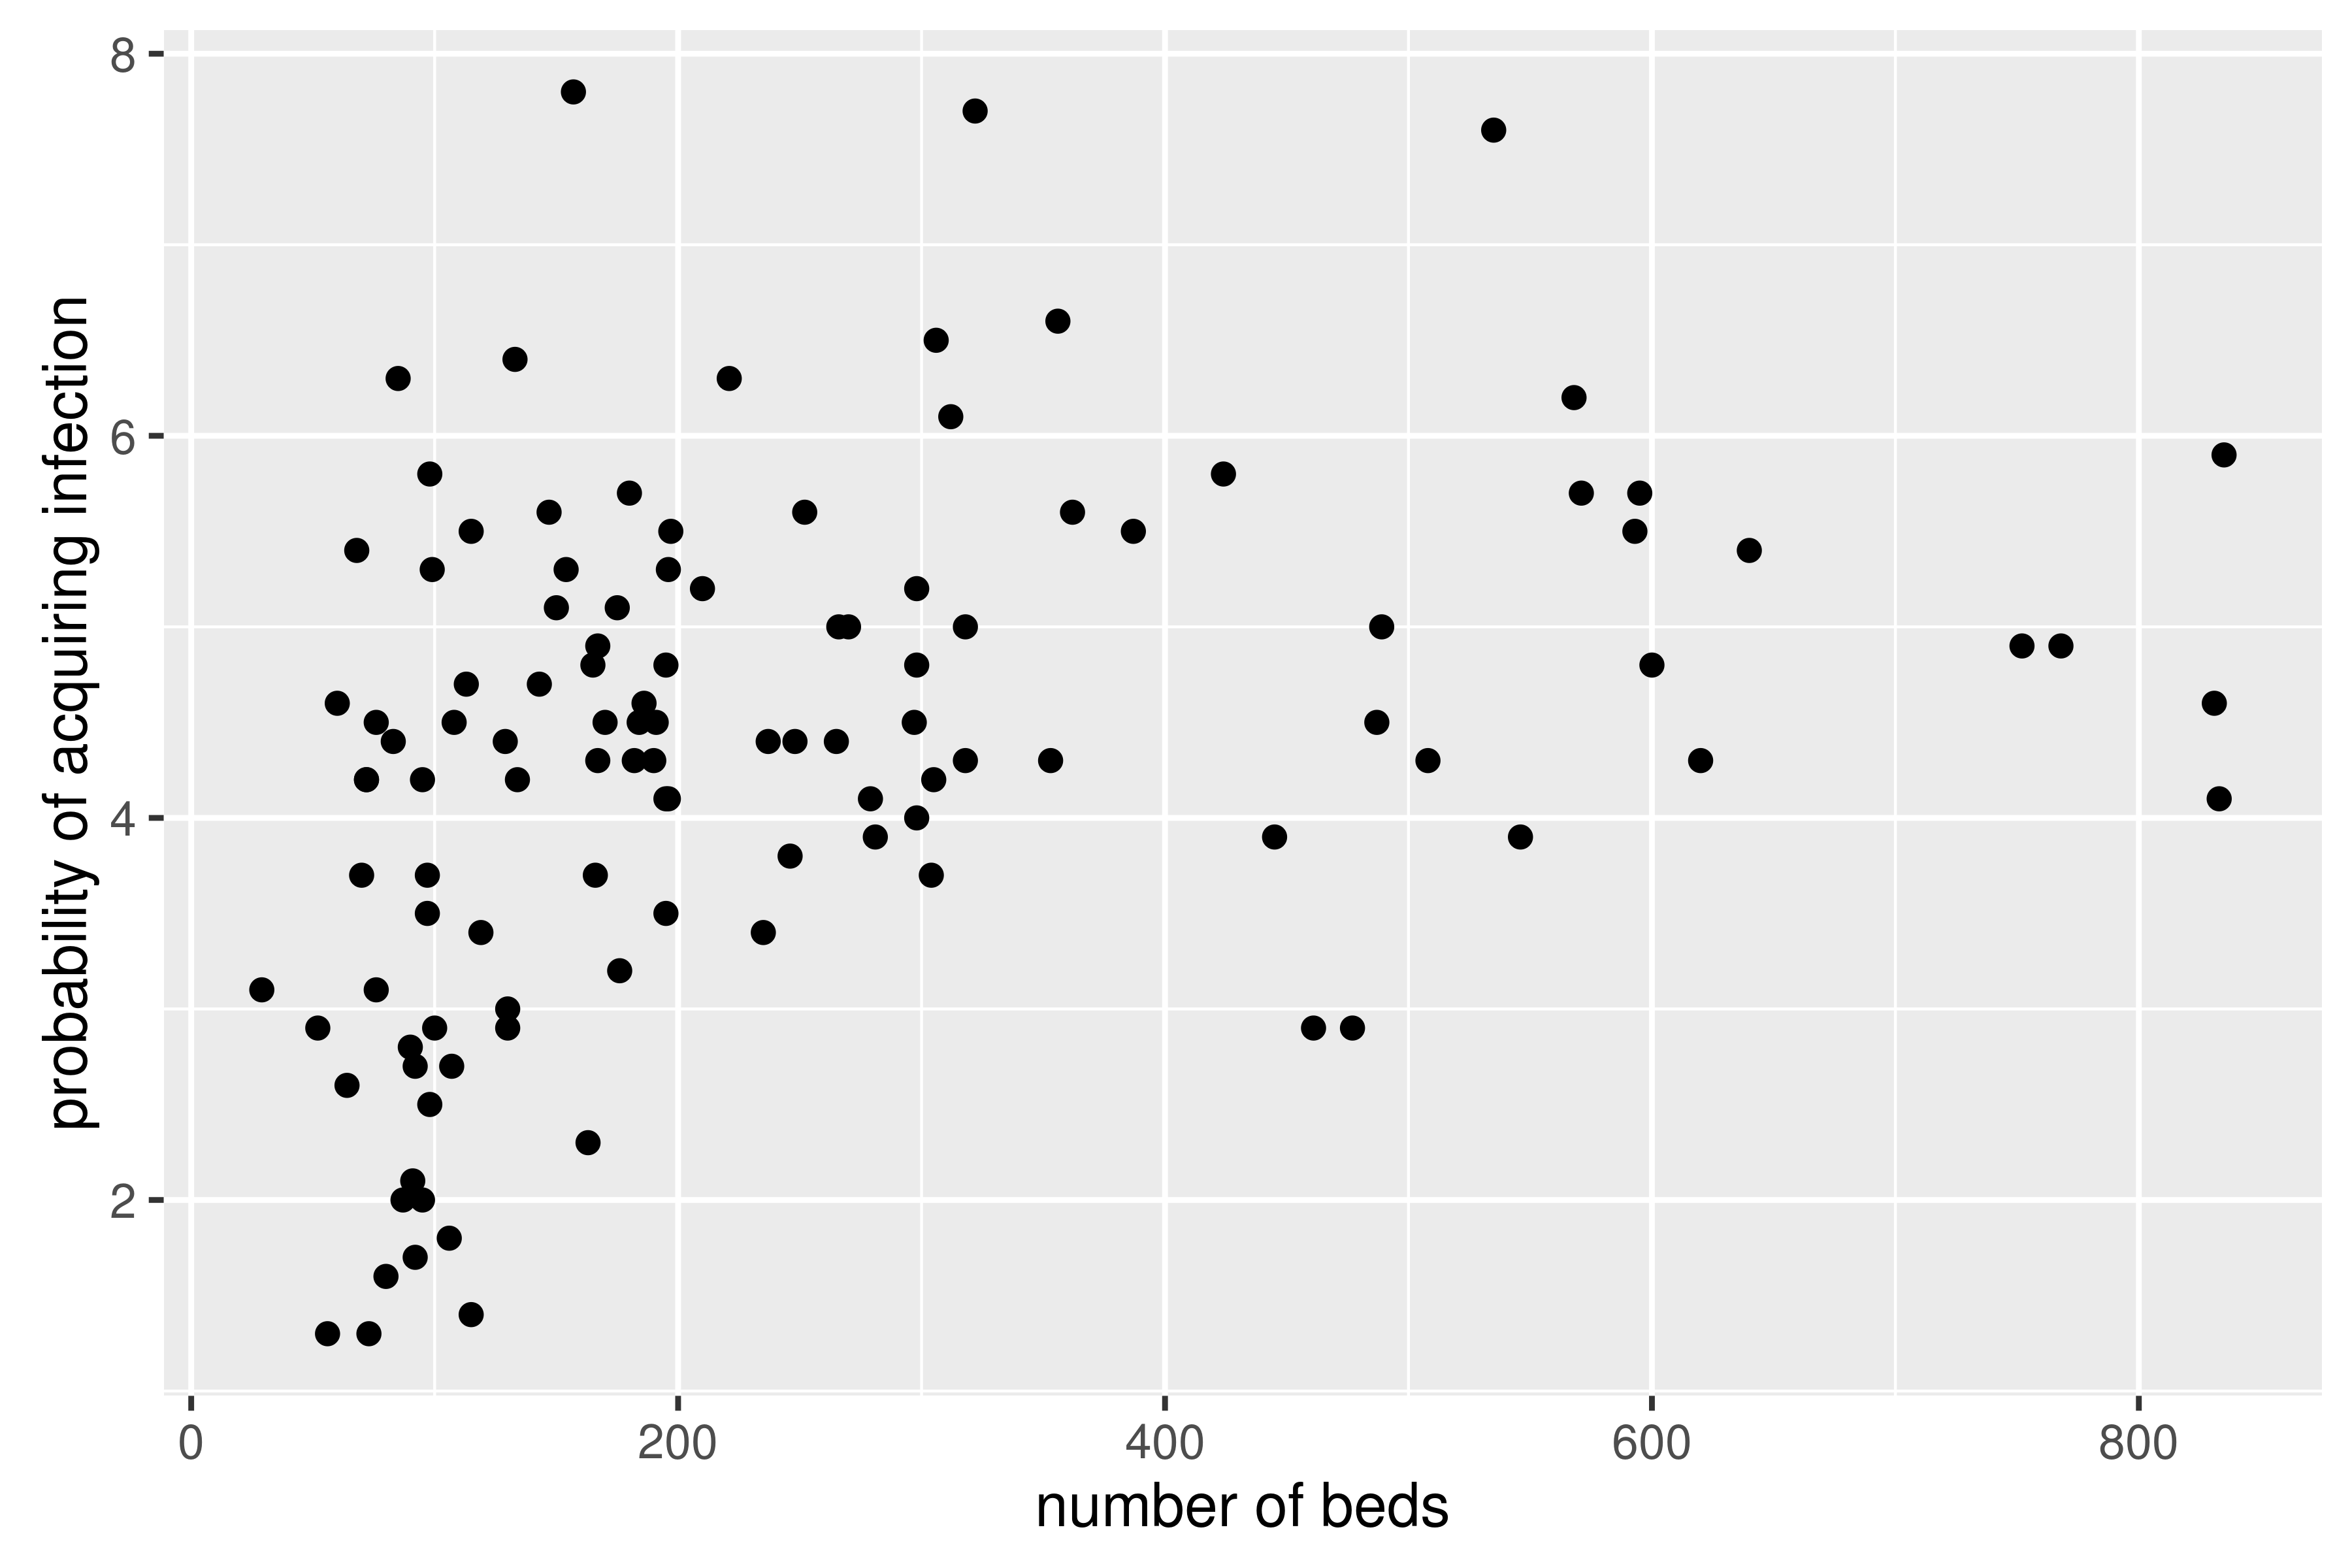
\includegraphics[width=1\textwidth]{scatter_plot_bed.png} \\
			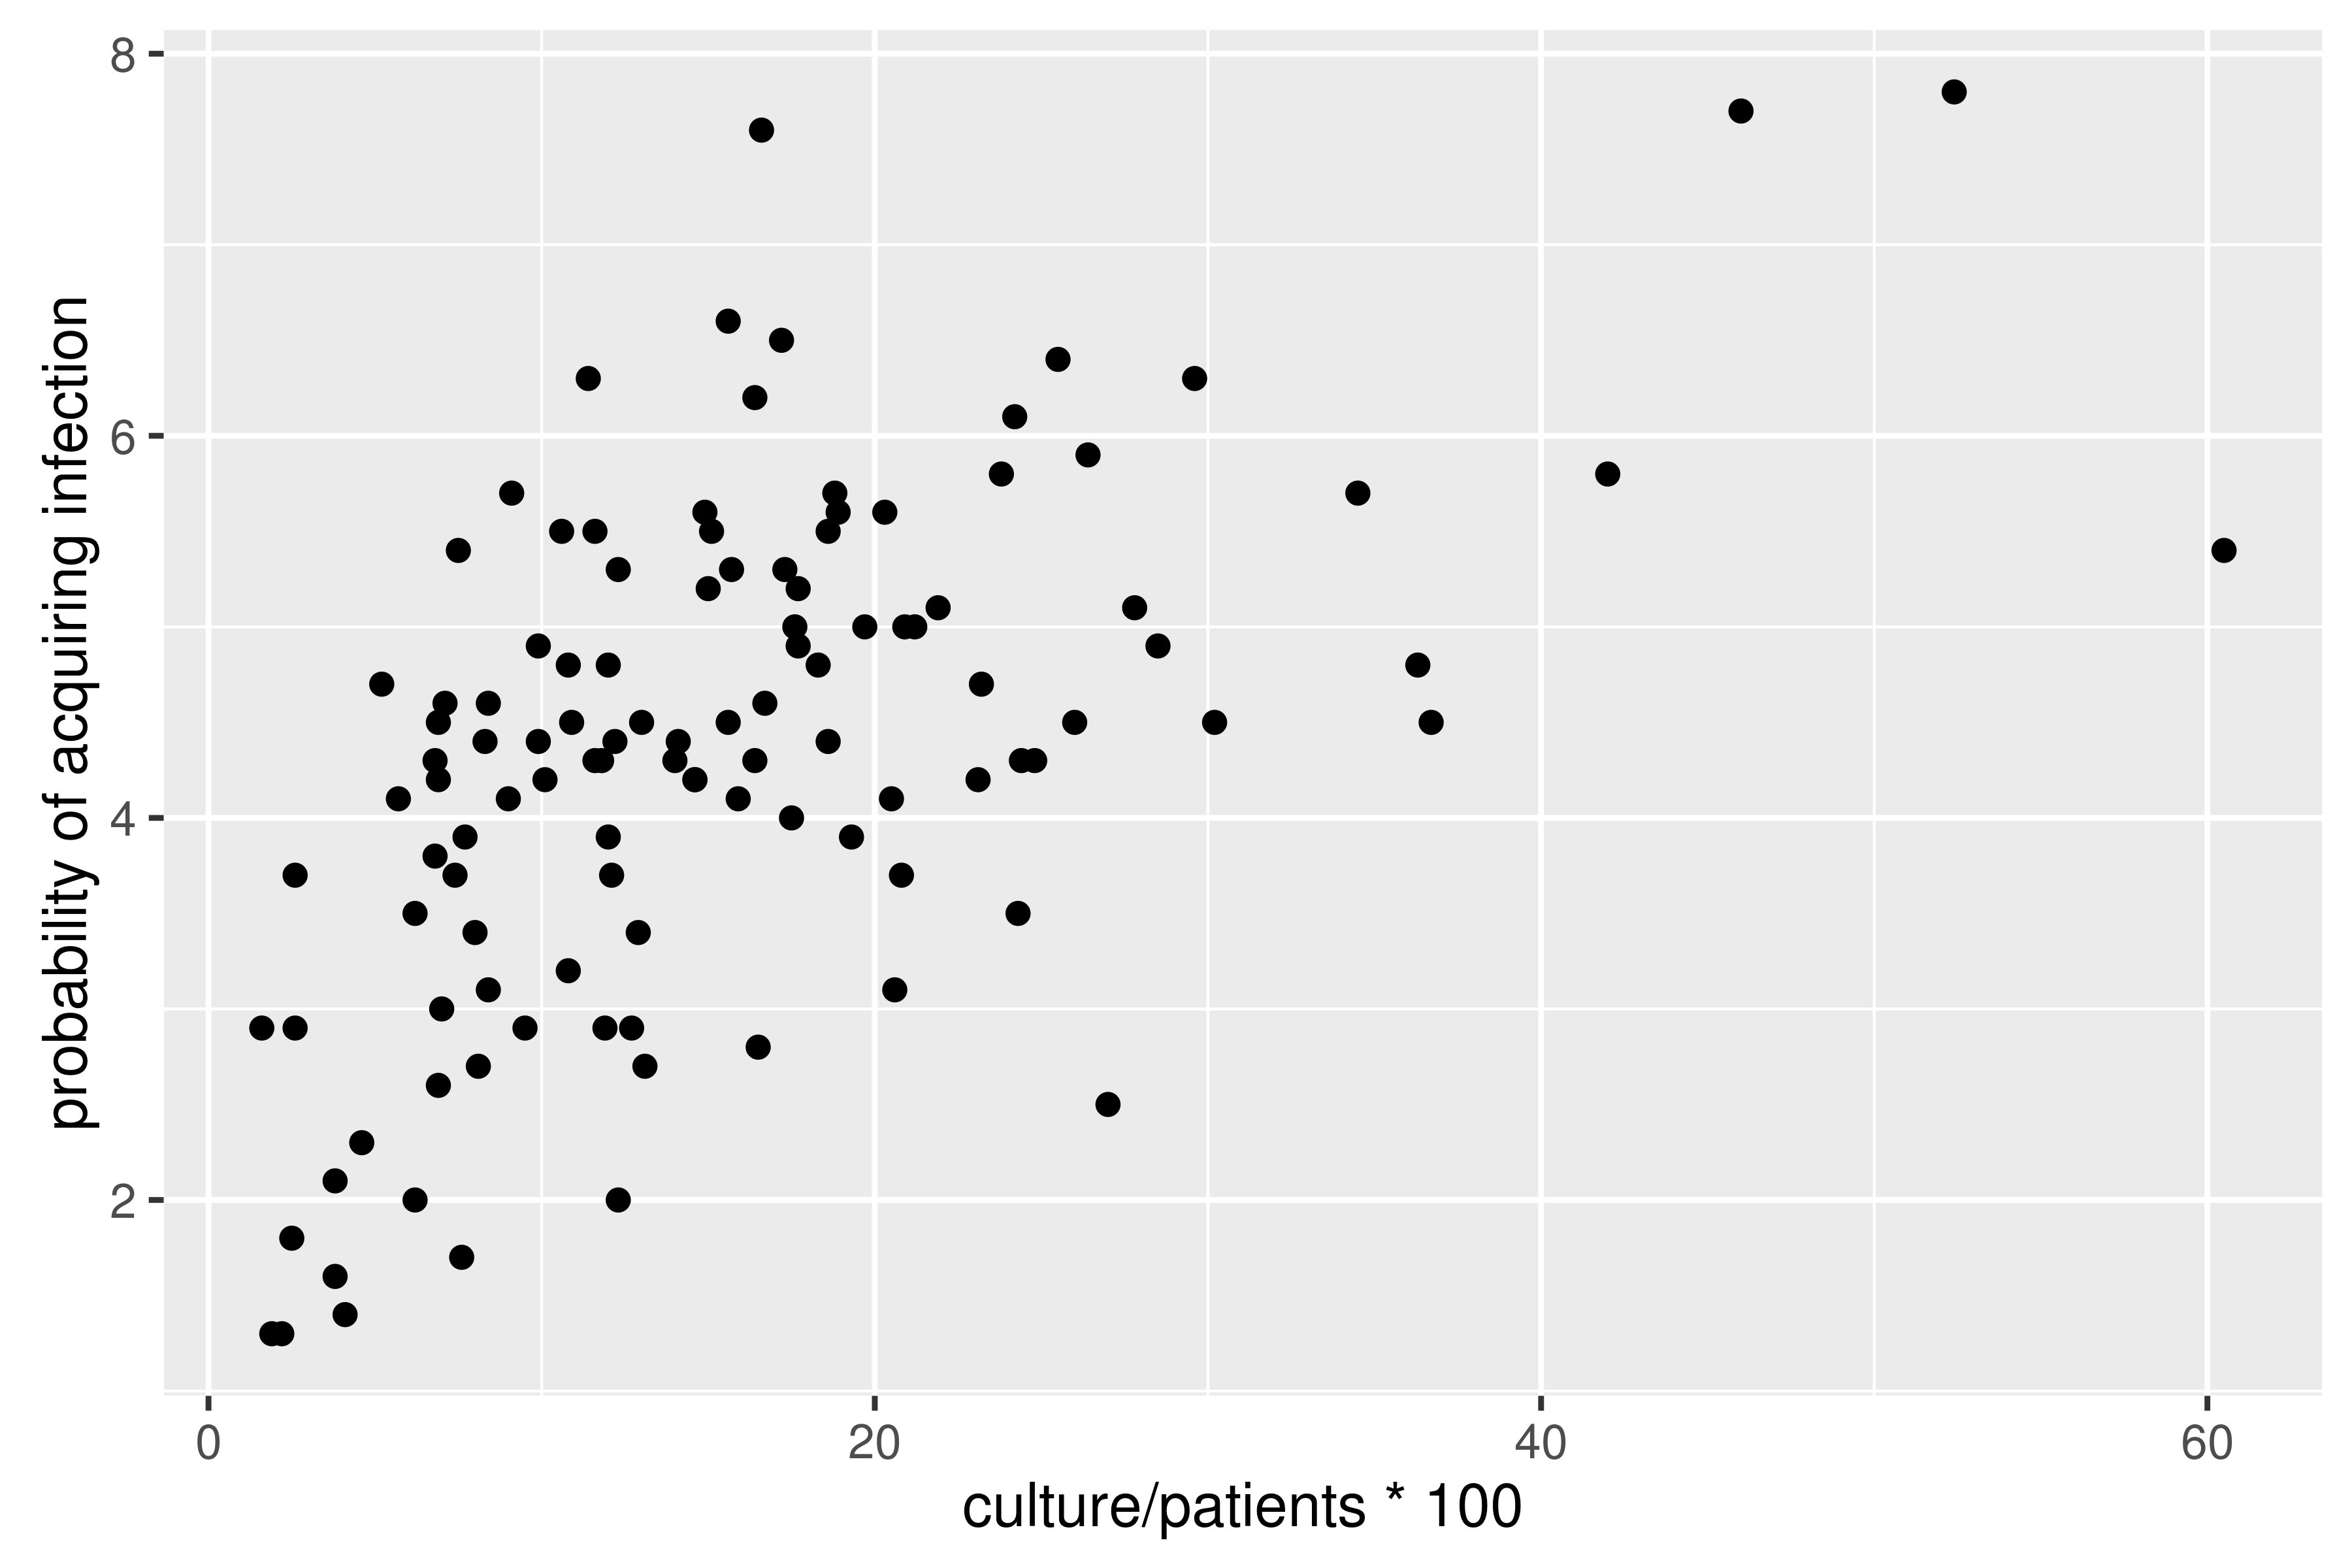
\includegraphics[width=1\textwidth]{scatter_plot_culture.png} 
		\end{minipage}
	}
	\subfigure{
		\begin{minipage}[b]{0.55\textwidth}
			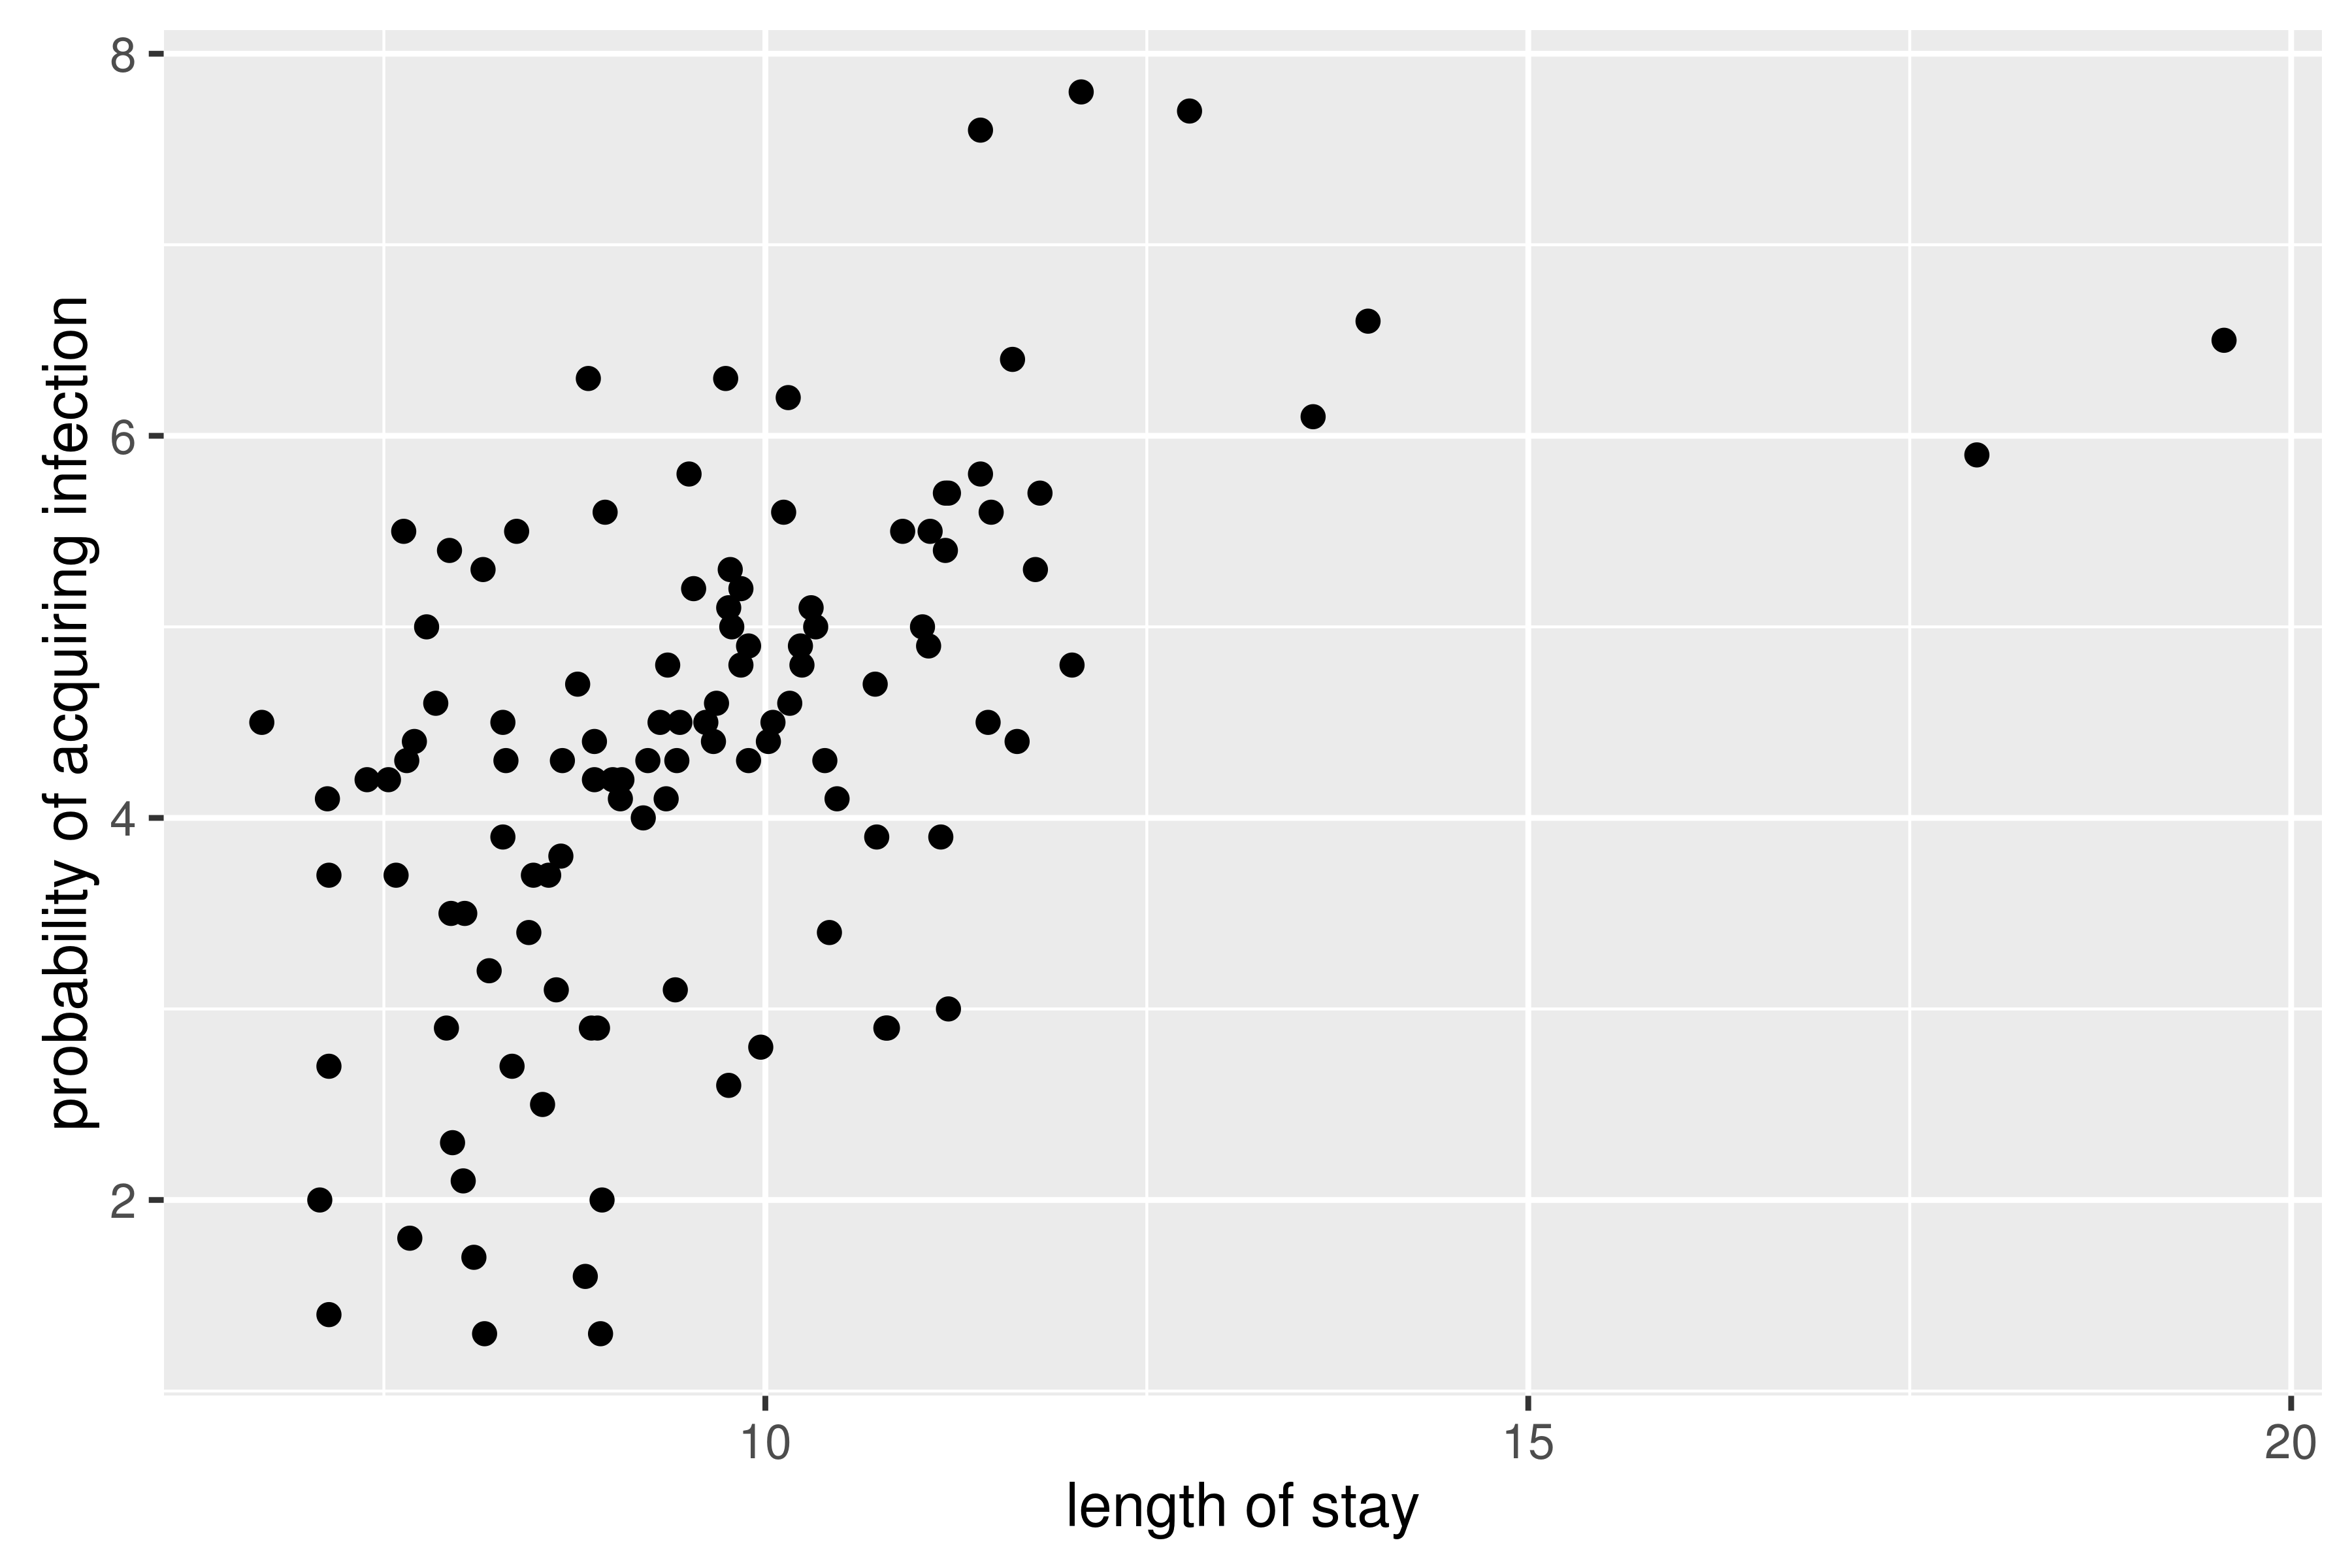
\includegraphics[width=1\textwidth,height=0.3\textheight]{scatter_plot_length.png} \\
		\end{minipage}
	}
\caption{Scatter plots of different numerical variables}
\end{figure}
\subsection{Five Number Summary}
Five statistics numbers give a brief review of basic information on our dataset. As shown in the table below, differences exist between varied categories, which suggests categorical variables are supposed to be included in the target model.
 \begin{table}[H]
	\centering
	\begin{tabular}{ccccccc}
		\midrule[1.5pt]
        Region &Min &$Q_1$ &Median&Mean &$Q_3$ &Max\\
        \hline
       NC   & 1.300       &3.8500     &4.400   &4.394      &5.225   &7.800\\
      NE    &2.500       &4.200     &4.850   &4.861      &5.750  &7.700\\
       S    &1.300       &2.900      &4.200    &3.927       &4.700  &7.600\\
      W    &2.600       &4.075      &4.450   &4.381      &4.850    &5.600\\
        
		\midrule[1.5pt]
	\end{tabular}
	\caption{Five number table of Region }
\end{table}
 \begin{table}[H]
	\centering
	\begin{tabular}{ccccccc}
		\midrule[1.5pt]
		Medschool &Min &$Q_1$ &Median&Mean &$Q_3$ &Max\\
		\hline
    N    &1.300       &3.400     &4.300  &4.224      &5.025    &7.800000\\
     Y    &2.900     & 4.500    & 5.000    &5.094       &5.700    &7.700\\
		\midrule[1.5pt]
	\end{tabular}
	\caption{Five number table of Medschool}
\end{table}

\section{Data Preparation}
Outliers are inevitable in any dataset, which have an effect on outcomes of coefficients and prediction. R is able to find and remove these values.
\subsection{Boxplots}
Outliers are apparent to pick out according to boxplots below.
\begin{figure}[H]
	\centering
	\subfigure[Boxplot by Meddschool]{
		\begin{minipage}[b]{0.43\textwidth}
			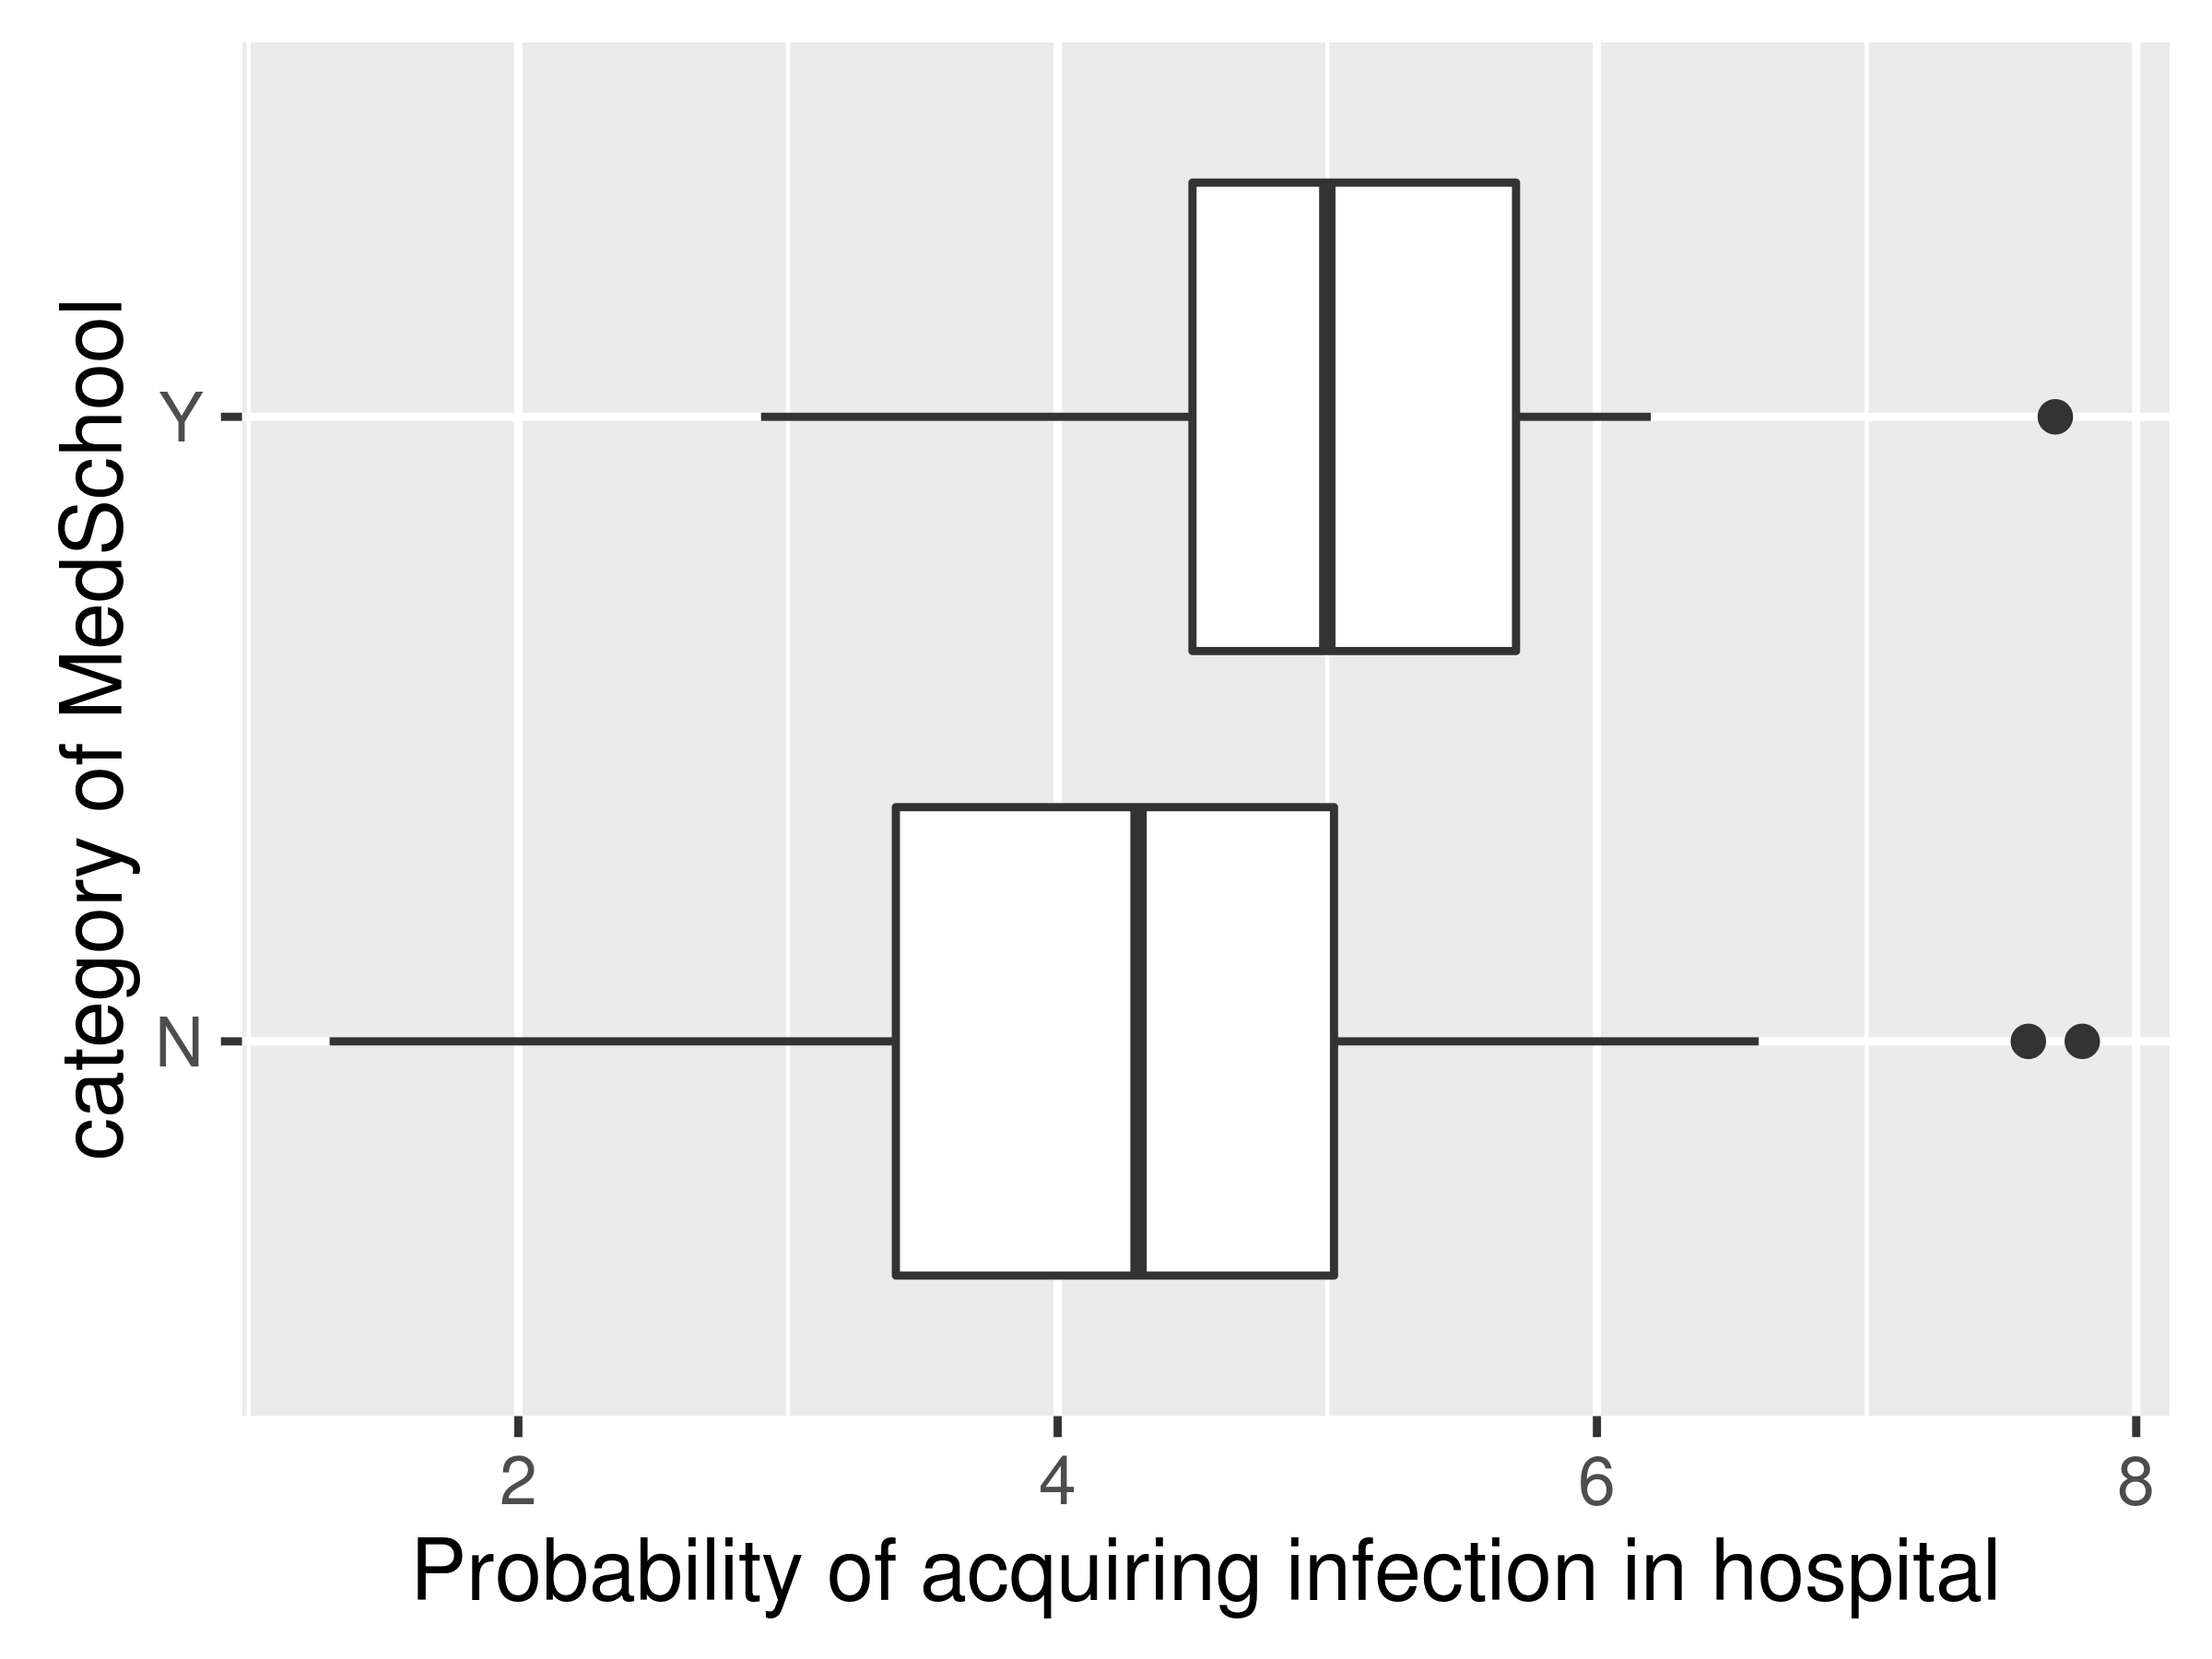
\includegraphics[width=1\textwidth]{group_boxplot_medschool.png} \\
		\end{minipage}
	}
	\subfigure[Boxplot by Region]{
		\begin{minipage}[b]{0.43\textwidth}
			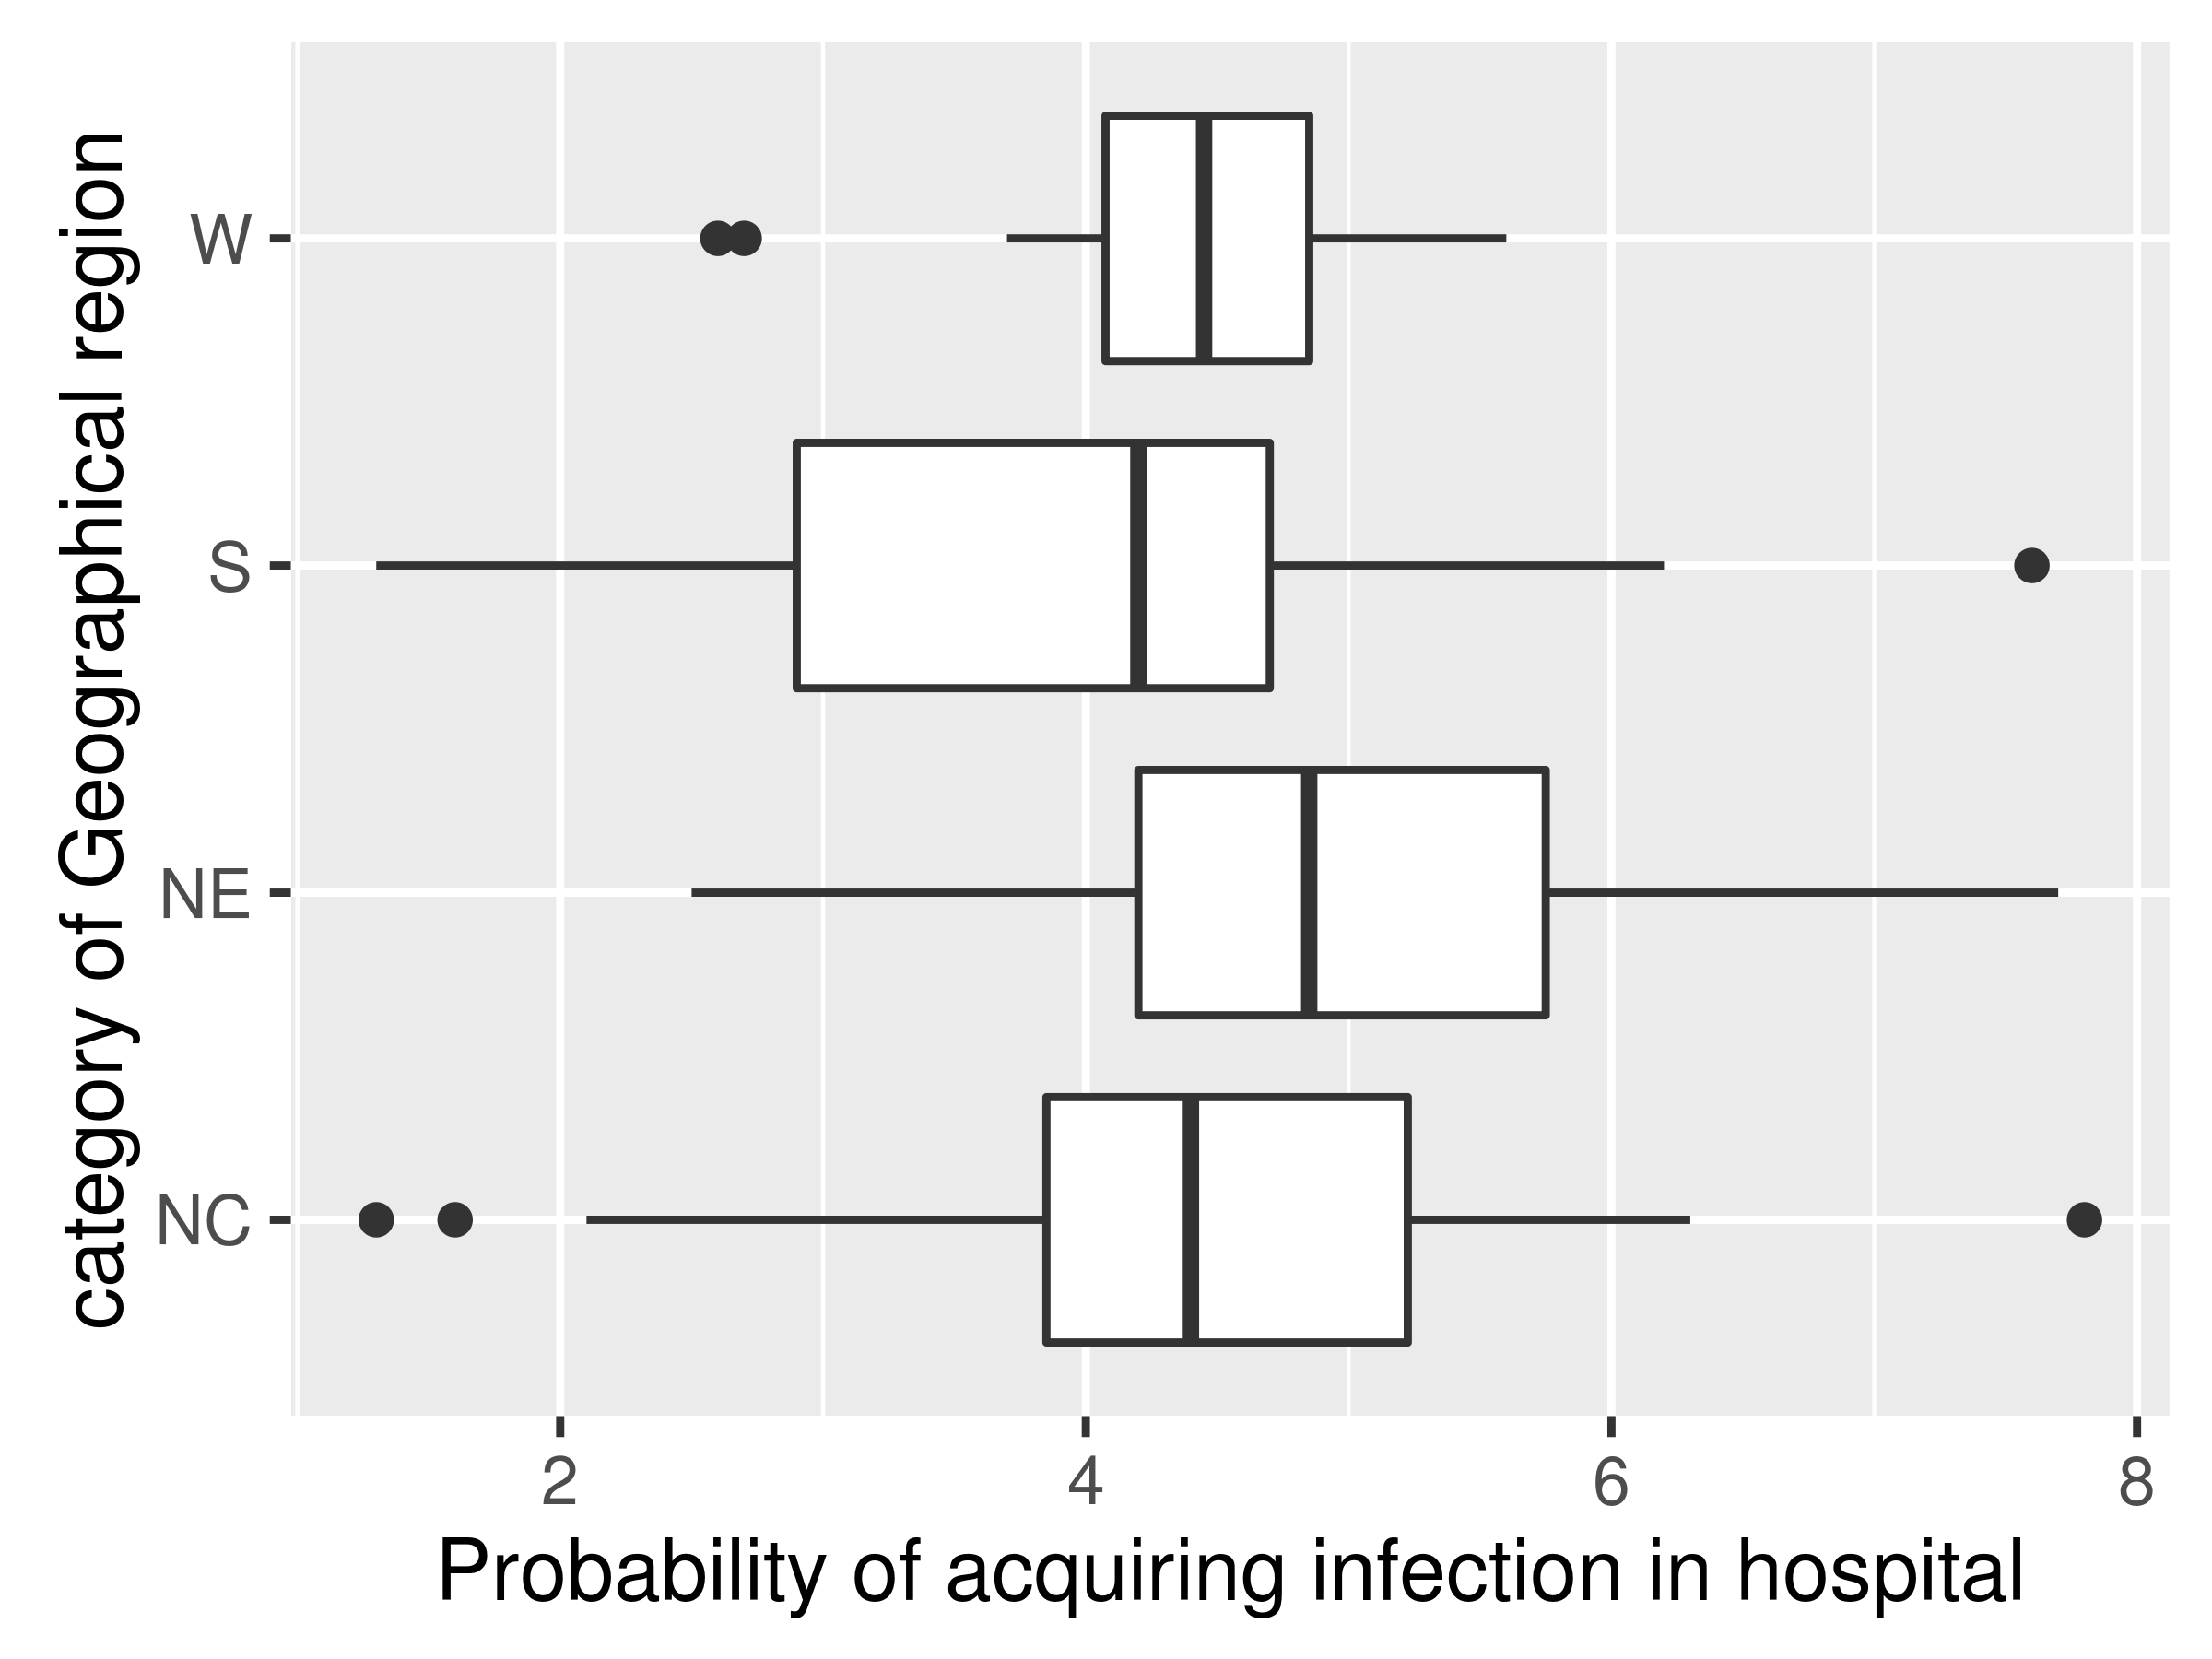
\includegraphics[width=1\textwidth]{group_boxplot_region.png} \\
		\end{minipage}
	}
	\caption{Boxplots by different categorical variables}
\end{figure}

\subsection{Remove Outliers}
We removed 10 outliers, the ratio of which to the number of samples in the whole dataset is 8.850\%, thus would not affect the dataset too much. Outliers are shown in the following table.
 \begin{table}[H]
	\centering
	\begin{tabular}{ccccccc}
		\midrule[1.5pt]
		Index & Length &Infect &Culture &Bed &MedSchool& Region\\
		\hline
	
        2    &8.82    &1.6     &3.8  &80         &N     &NC\\
		8  &11.18    &5.4    &60.5 &640         &Y     &NC\\
	    13  &12.78    &7.7      &46 &322         &Y    &NE\\
	    47   &19.56   & 6.5    &17.2 &306         &N     &NE\\
	    53  &11.41    &7.6    &16.6 &535         &N      &S\\
	    54  &12.07   & 7.8    &52.4 &157         &N     &NC\\
	    93   &8.92   & 1.3     &2.2  &56         &N     &NC\\
	 	101  & 9.76  &  2.6     &6.9  &64         &N      &W\\
	    103   &7.14  &  2.7    &13.1  &92        & N      &W\\
	    112  &17.94  &  5.9    &26.4 &835         &Y     &NE\\
		\midrule[1.5pt]
	\end{tabular}
	\caption{Detailed information of outliers }
\end{table}
\section{Model Fitting}
\subsection{Model Selection}
The ``correct" model can be found based on the criatia of A.I.C or B.I.C. R gives us two candidate models without considering any interaction term.\par 
We found that the full model has the lowest A.I.C. compared to all subset models. Therefore, the first model we built is
\begin{equation}
\begin{split}
\hat{y_1}= &-0.4536+0.3962X_1+0.0586X_2+0.0013X_3-0.4005X_{4Y}\\ &-0.4577X_{5NE}-0.3619X_{5S}+0.9163X_{5W}
\end{split}
\end{equation} \par
We also found that the model with the lowest B.I.C. compared to all other models. Therefore, the second model we built is
\begin{equation}
\begin{split}
\hat{y_2}= &-0.5573+0.4389X_1+0.0565X_2\\&-0.5097X_{5NE}     -0.3471X_{5S}+0.9048X_{5W} 
\end{split}
\end{equation}
Because A.I.C usually provides us with a larger "correct" model while B.I.C usually favors the "smaller" one, we were able to find our final model somewhere between the first model based on A.I.C and the second model based on B.I.C. Using some techniques to compare different models is of great necessity, as what we did in the next.
\subsection{C.I. \& H.T. for $\beta_i$}
Because the first model is larger than the second one, at the same time, a ``correct" model is needed in the end. By analyzing C.I. and H.T. of $\beta$s, we could decide whether we should drop some variables from the first model.
\begin{table}[H]
	\centering
	\begin{tabular}{ccc}
		\midrule[1.5pt]
		& 2.5 \% &97.5 \% \\
		\hline
		(Intercept) &-1.8014 &0.8942\\
		$X_1$         &  0.2507 &0.5417\\
		$X_2$           &0.0371 &0.0802\\
		$X_3$           &0.0001 &0.0024\\
		$X_{4Y}$         &-0.9805 &0.1796\\
		$X_{5NE}$        &-0.9469 &0.0316\\
		$X_{5S}$         &-0.7823 &0.0585\\
		$X_{5W}$          &0.3422 &1.4905\\	
		\midrule[1.5pt]
	\end{tabular}
	\caption{C.I. of $\beta s$ of the first model }
\end{table}
We were considering to drop $X_4$ at this moment since confidence intervals containing 0 do not suggest a significant relationship with the response variable $Y$. Though indicate variables like $X_{5NE}$ and $X_{5S}$ contain 0 as well, we could not drop $X_5$ from the first model because $X_{5W}$ does not contain 0 and suggests a strong relationship with $Y$.
\begin{table}[H]
	\centering
	\begin{tabular}{ccccc}
		\midrule[1.5pt]	
		&Coefficients
		&Estimate Std. Error &$t$ value &Pr($>|t|$)\\
		\hline    
	  (Intercept) &-0.453605 &  0.678888 & -0.6680 &0.50565    \\
		$X_1$          & 0.396160  & 0.073290   &5.405 &4.79e-07\\
		$X_2$          & 0.058650  & 0.010860   &5.401 &4.89e-07\\
		$X_3$          & 0.001265   &0.000568   &2.227  &0.02833 \\
		$X_{4Y}$         &-0.400484   &0.292175  &-1.371  &0.17370  \\  
		$X_{5NE}$        &-0.457657  & 0.246435  &-1.857  &0.06639 \\
		$X_{5S}$         &-0.361916   &0.211761  &-1.709  &0.09070 \\
		$X_{5W}$         & 0.916322   &0.289204   &3.168  &0.00206 \\
		\midrule[1.5pt]
	\end{tabular}
	\caption{H.T. for $\beta s$ of the first model }
\end{table}
The p-value of $\beta_4$ is big enough for us to accept $H_0$ which means $\beta_4=0$, so we could drop $X_4$. Now we have a new candidate model `` $Y \sim X_1,X_2,X_3,X_5$" and dismiss the full one.
\subsection{Partial $R^2$}
We found that the value of $\beta_3$ is quite small. We used partial $R^2$ to estimate how much error we could reduce by adding $X_3$ to our second model ``$Y\sim X_1,X_2,X_5$". If partial $R^2$ is small, we would consider dropping $X_3$.
\begin{equation}
R^2\{X_1,X_2,X_3,X_5|X_1,X_2,X_5\}=\frac{SSE_{S}-SSE_{L}}{SSE_{S}}=3.156\%
\end{equation}
$R^2\{X_1,X_2,X_3,X_5|X_1,X_2,X_5\}$ is not large enough to overweigh the additional cost a large model will bring about. Besides, considering  the correlation coefficient between $X_3$ and $Y$ and the scatter plot of $X_3$ and $Y$ in section 2.2 only suggests a weak relationship,  we dropped $X_3$ and chose the second model ``$Y\sim X_1,X_2,X_5$" temporarily as our final model.
\subsection{Add Interaction Terms}
At last, to figure out whether interaction terms should be added, we analyzed the C.I. of $\beta$s of relavant interaction terms and found that there was no need to add these terms because the C.I. all contain 0.
\begin{table}[H]
	\centering
	\begin{tabular}{ccc}
		\midrule[1.5pt]	
						&2.5 \% &97.5\% \\
		\hline    
		(Intercept) &-2.2187 &3.2553\\
		$X_1$           &0.0451 &0.6108\\
		$X_2$           &0.0336 &0.0778\\
		$X_{5NE}$        &-5.7841 &1.3486\\
		$X_{5S}$         &-5.6676 &1.3708\\
		$X_{5W}$         &-2.3968 &7.2876\\
		$X_1:X_{5NE}$     &-0.1829 &0.5292\\
		$X_1:X_{5S}$      &-0.1798 &0.5627\\
		$X_1:X_{5W}$      &-0.7801 &0.3557\\
		\midrule[1.5pt]
	\end{tabular}
	\caption{H.T. for $\beta s$ of interaction terms with $X_1$ }
\end{table}
\begin{table}[H]
	\centering
	\begin{tabular}{ccc}
		\midrule[1.5pt]	
		&2.5 \% &97.5\% \\
		\hline    
		(Intercept) &-1.5605  &1.3035\\
		$X_1$          &0.2868  &0.5552\\
		$X_2$          &-0.00532  &0.0815\\
		$X_{5NE}$        &-1.7807  &0.4531\\
		$X_{5S}$         &-1.8586 &-0.1378\\
		$X_{5W}$        & 0.1689  &2.6083\\
		$X_2:X_{5NE}$     &-0.0452  &0.0732\\
		$X_2:X_{5S}$      &-0.0068 &0.1038\\
		$X_2:X_{5W}$      &-0.1208  &0.0405\\
		\midrule[1.5pt]
	\end{tabular}
	\caption{H.T. for $\beta s$ of interaction terms with $X_2$ }
\end{table}
\subsection{Final Model}
Based on the discussion above, we have found the most important variables $X_1,X_2,X_5$ and reached our final model ``$Y\sim X_1+X_2+X_5$".

\section{Model Diagnostics}
There are a few assumptions we have to obey when using linear regression. Mostly, we care about the normality of $e_i$ and whether the variance is constant.
\begin{figure}[htbp]
	\centering
	\subfigure[Normal qqplot]{
		\begin{minipage}[b]{0.43\textwidth}
			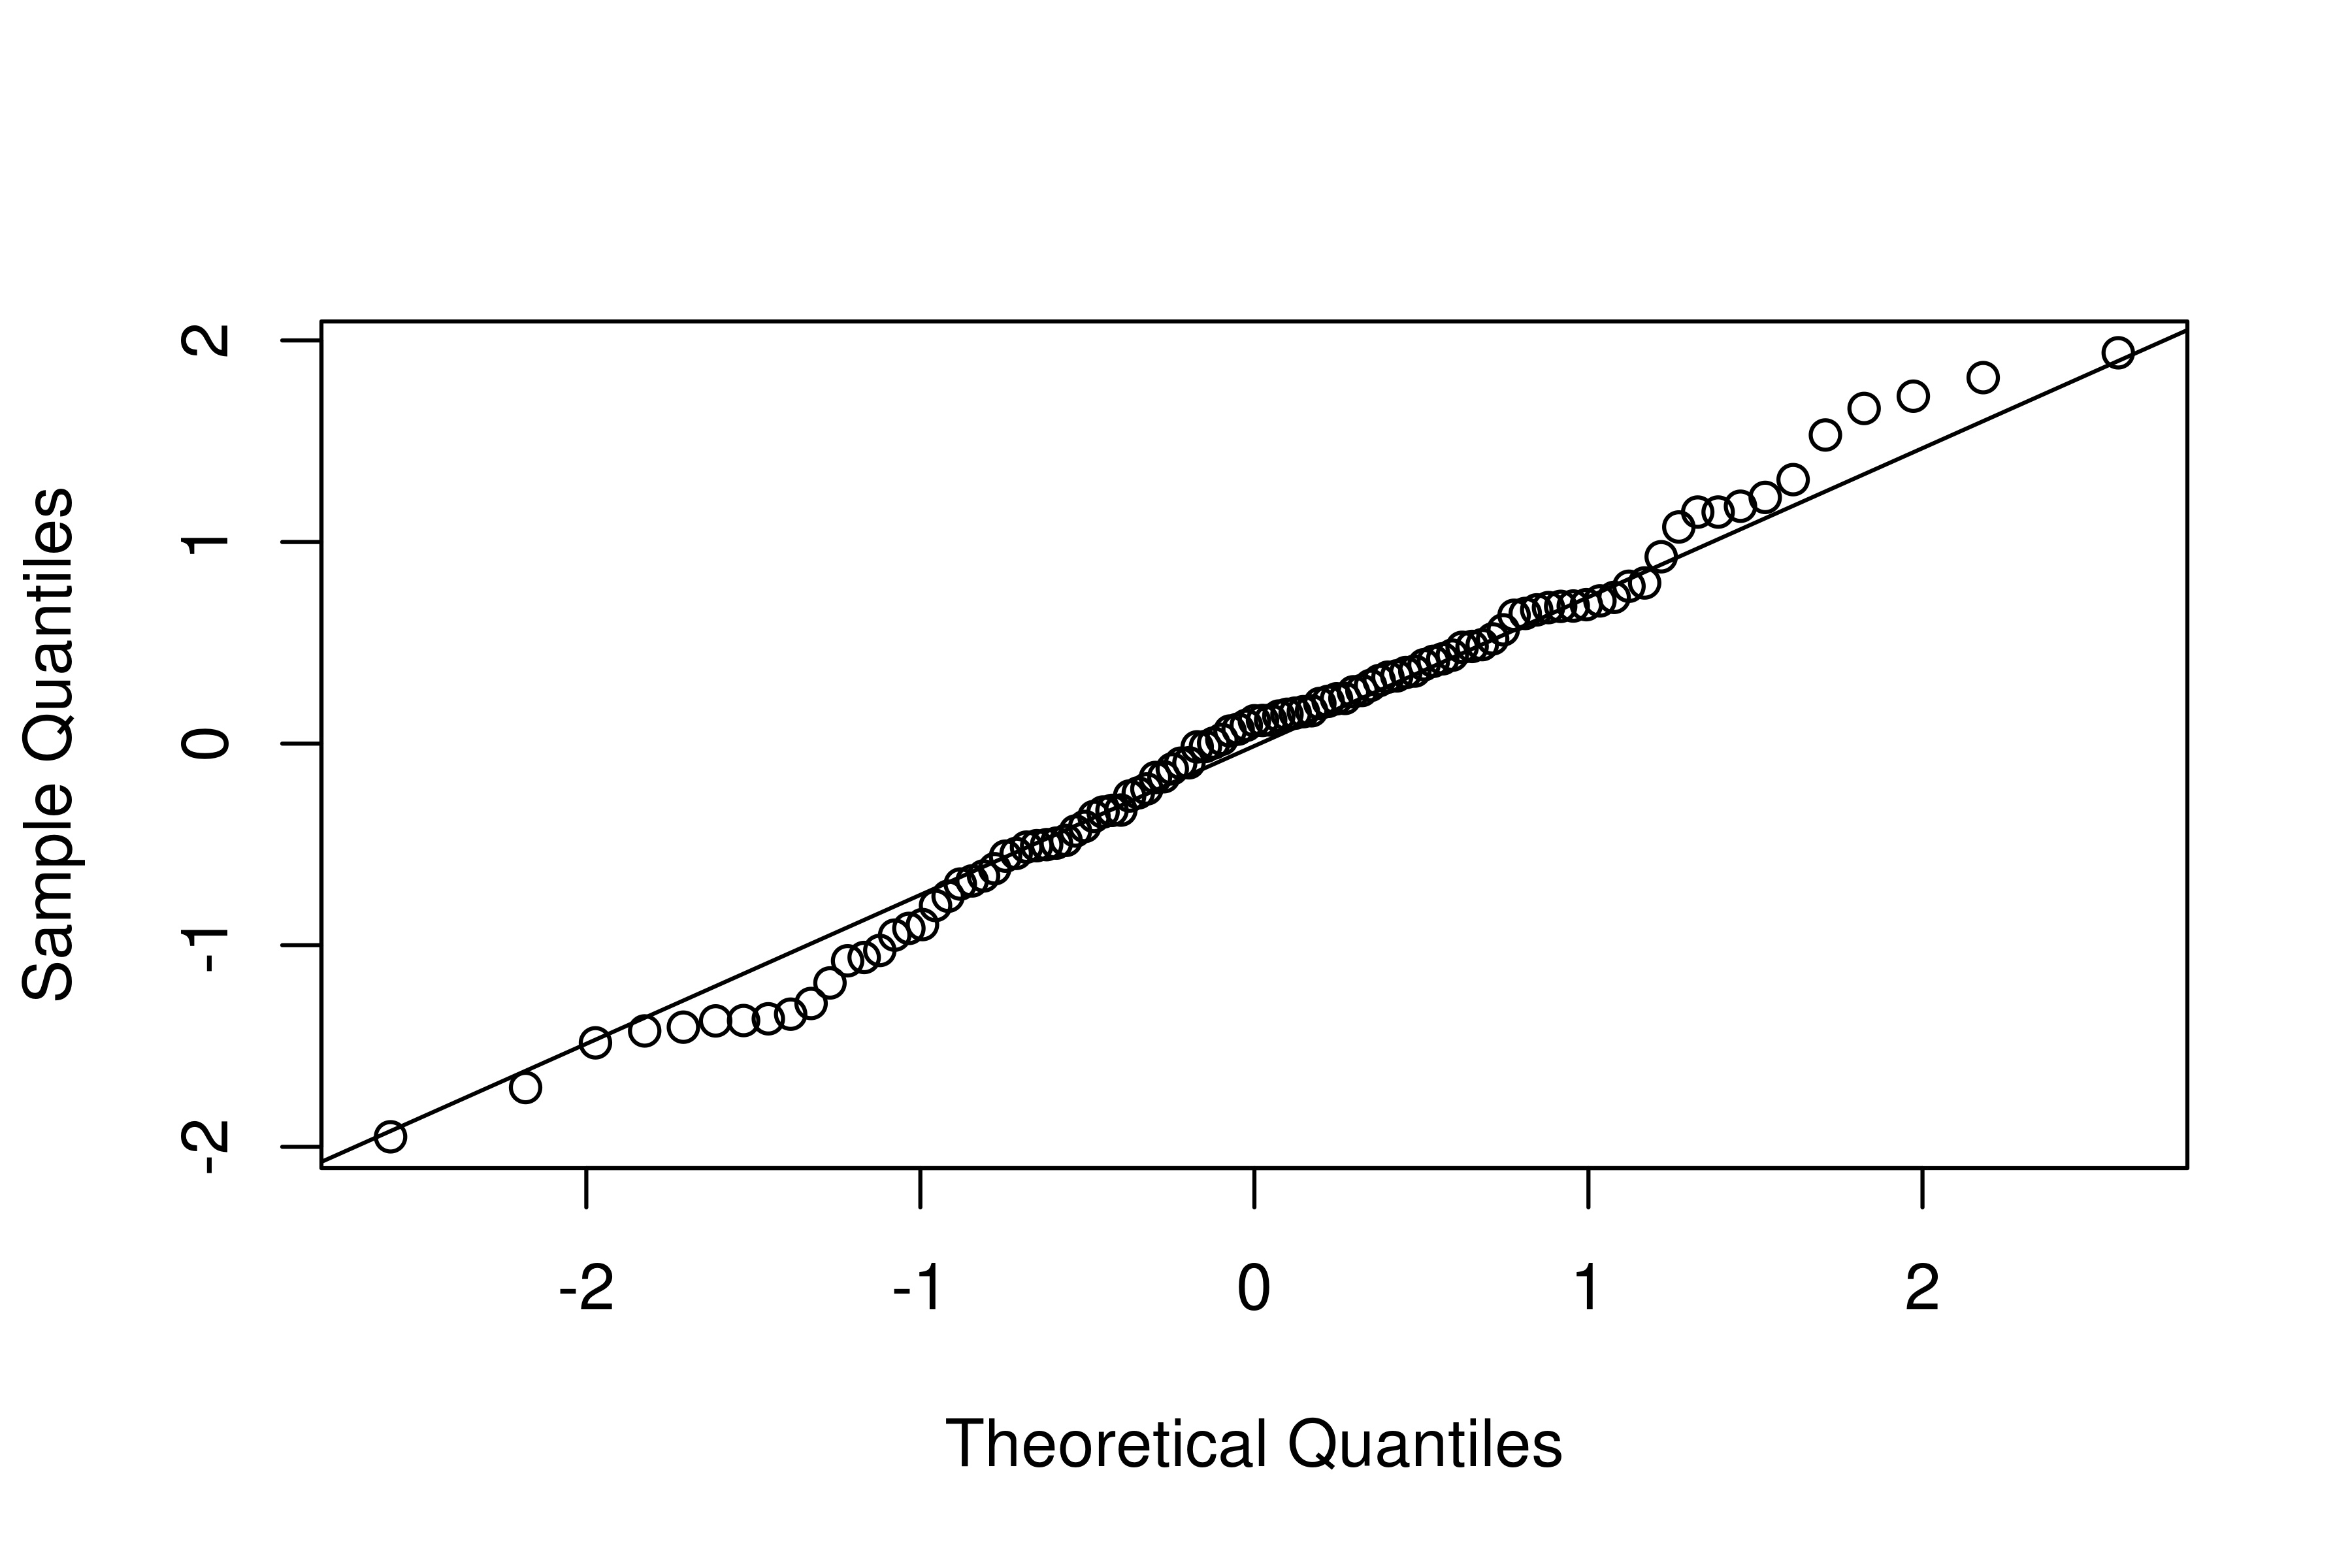
\includegraphics[width=1\textwidth,height=0.25\textheight]{qqplot.jpg} \\
		\end{minipage}
	}
	\subfigure[$e_i$ v.s. $\hat{y_i}$ plot]{
		\begin{minipage}[b]{0.43\textwidth}
			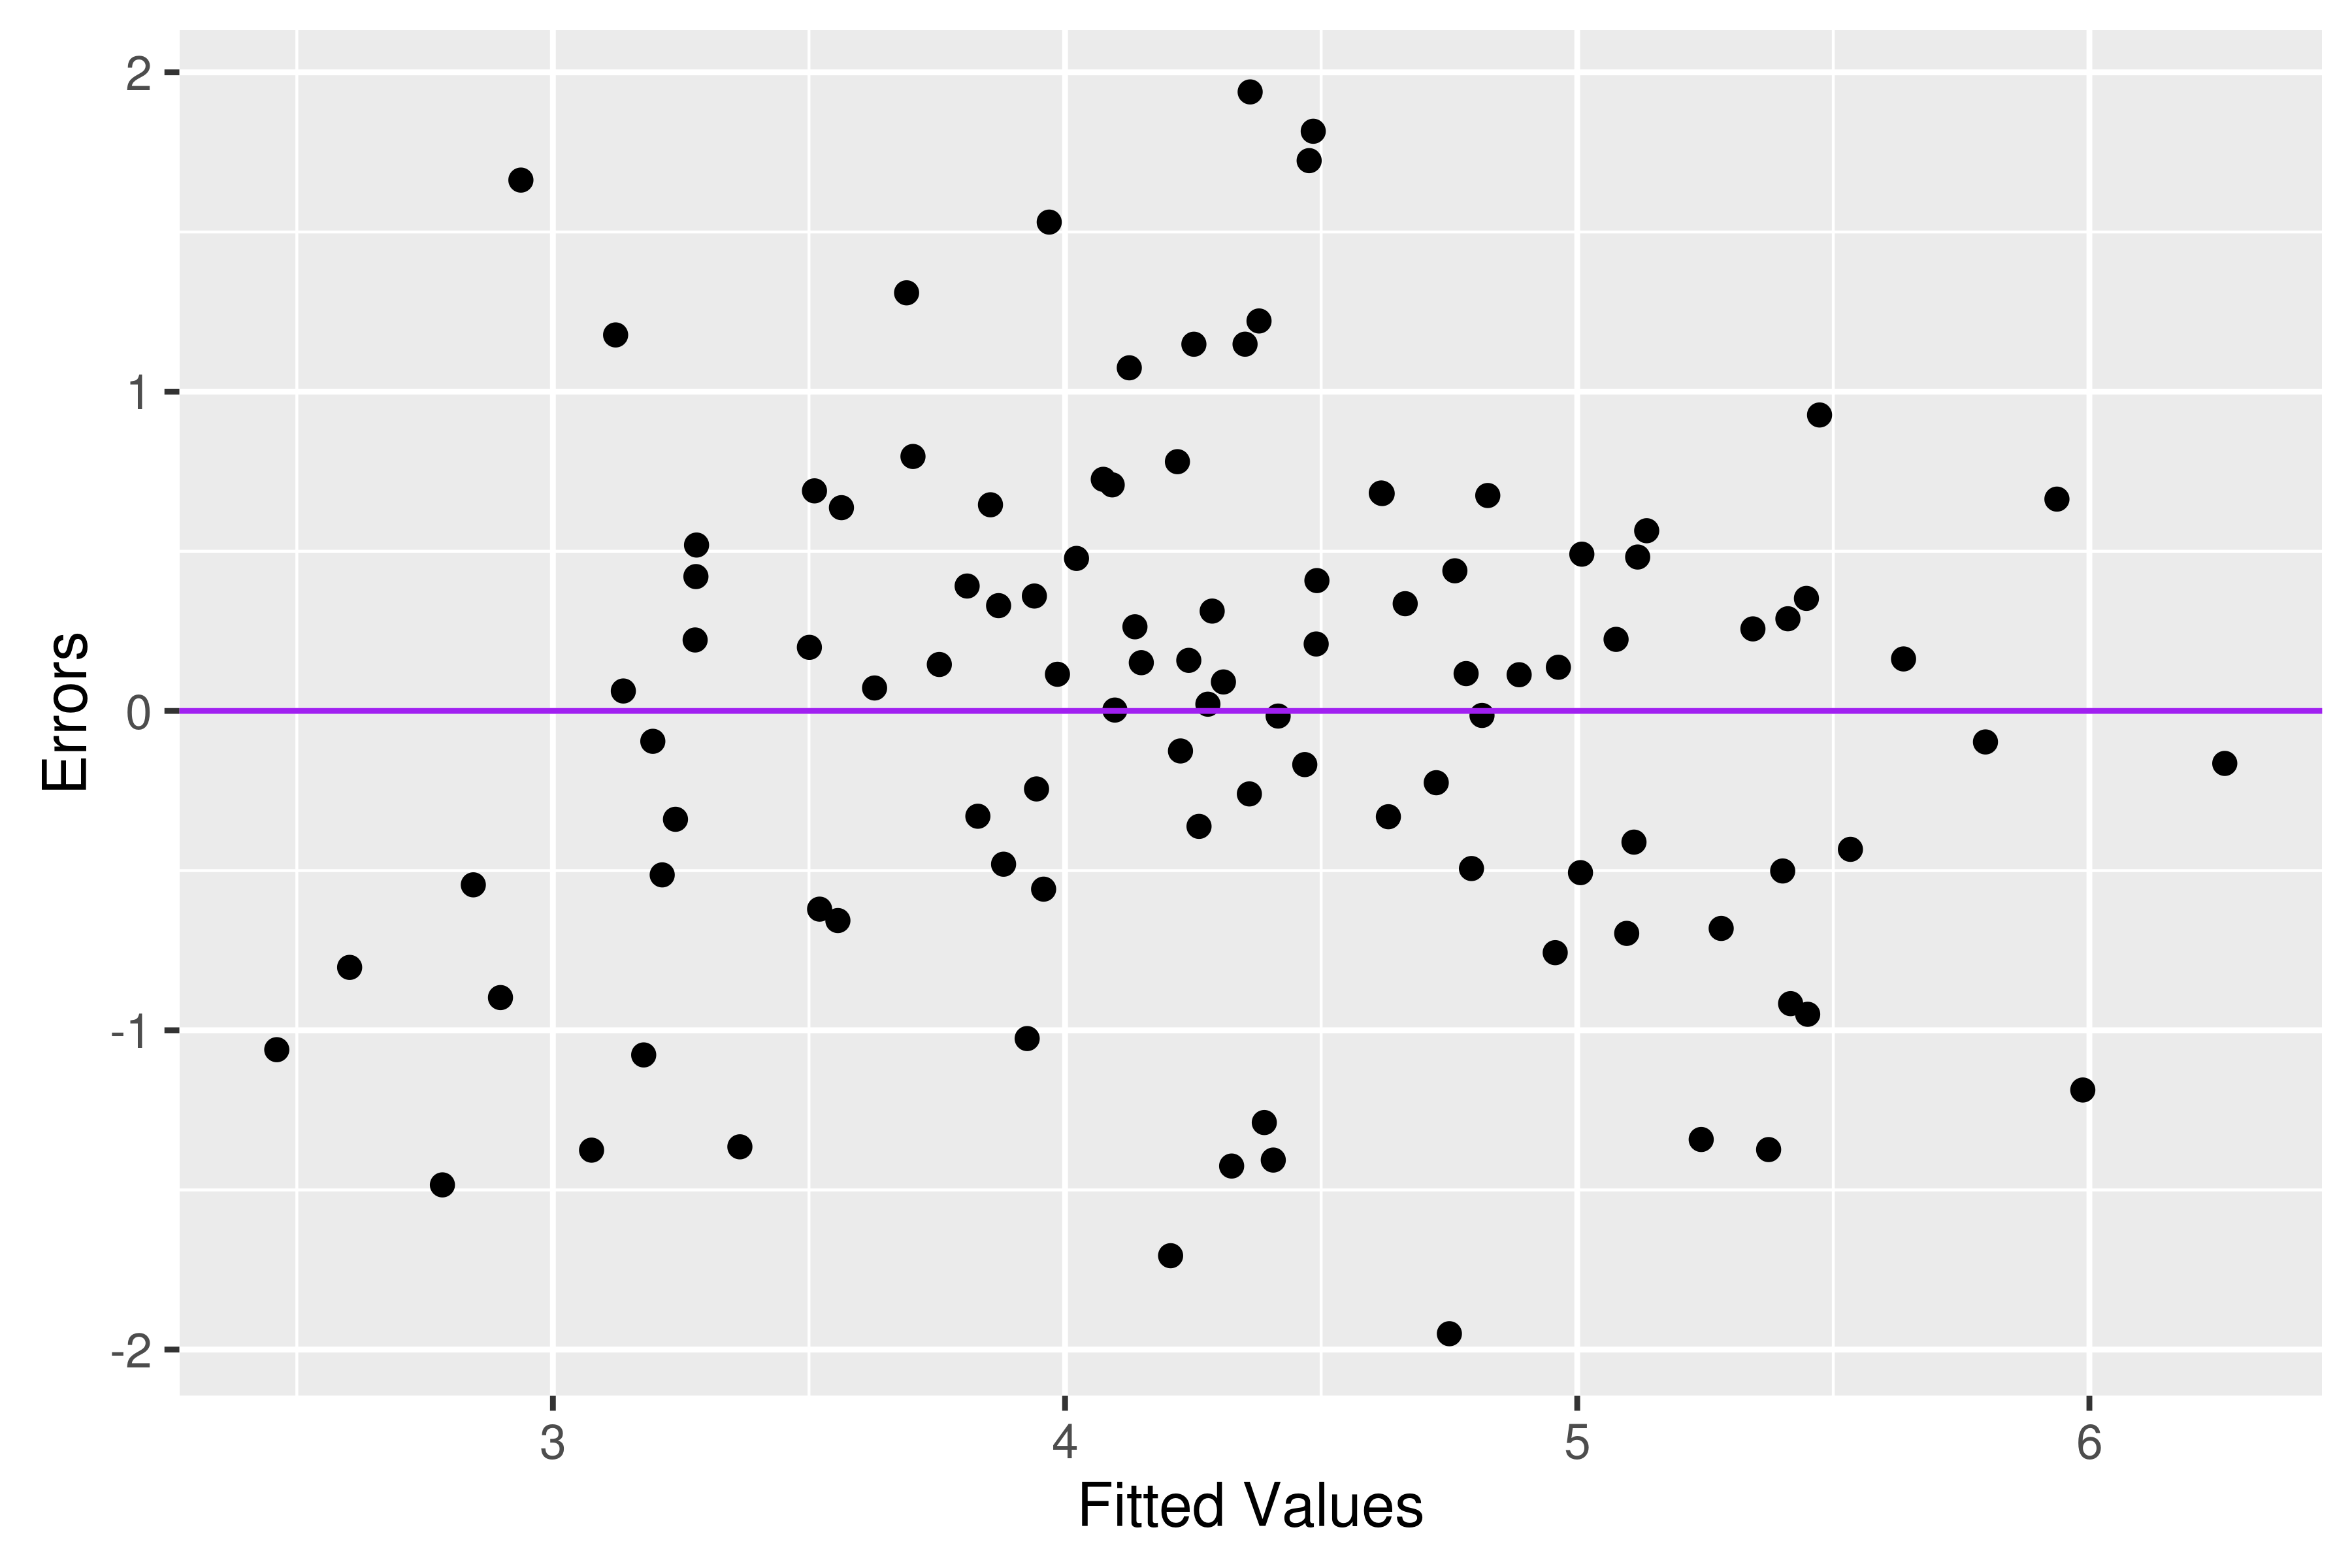
\includegraphics[width=1\textwidth]{scatter_plot_constant_variance.png} \\
		\end{minipage}
	}
	\caption{Plots of model diagnostics}
\end{figure}
\subsection{$e_i$ Normality}
The assumption is that $\varepsilon\sim \mathcal N(0,\sigma_{\varepsilon})$ in linear regression. We use $e_i$ to estimate $\varepsilon$ in practice. There are two popular ways to verify this assumption, which are QQ plot and Shapiro-Wilk Normality Test.
\subsubsection{QQ Plot}
Accoding to the figure in Figure3(a), except several deviations, most points are near the expected line $y=x$, which suggests $e_i$ is normally distributed.
% \begin{figure}[H]
%	\centering
%	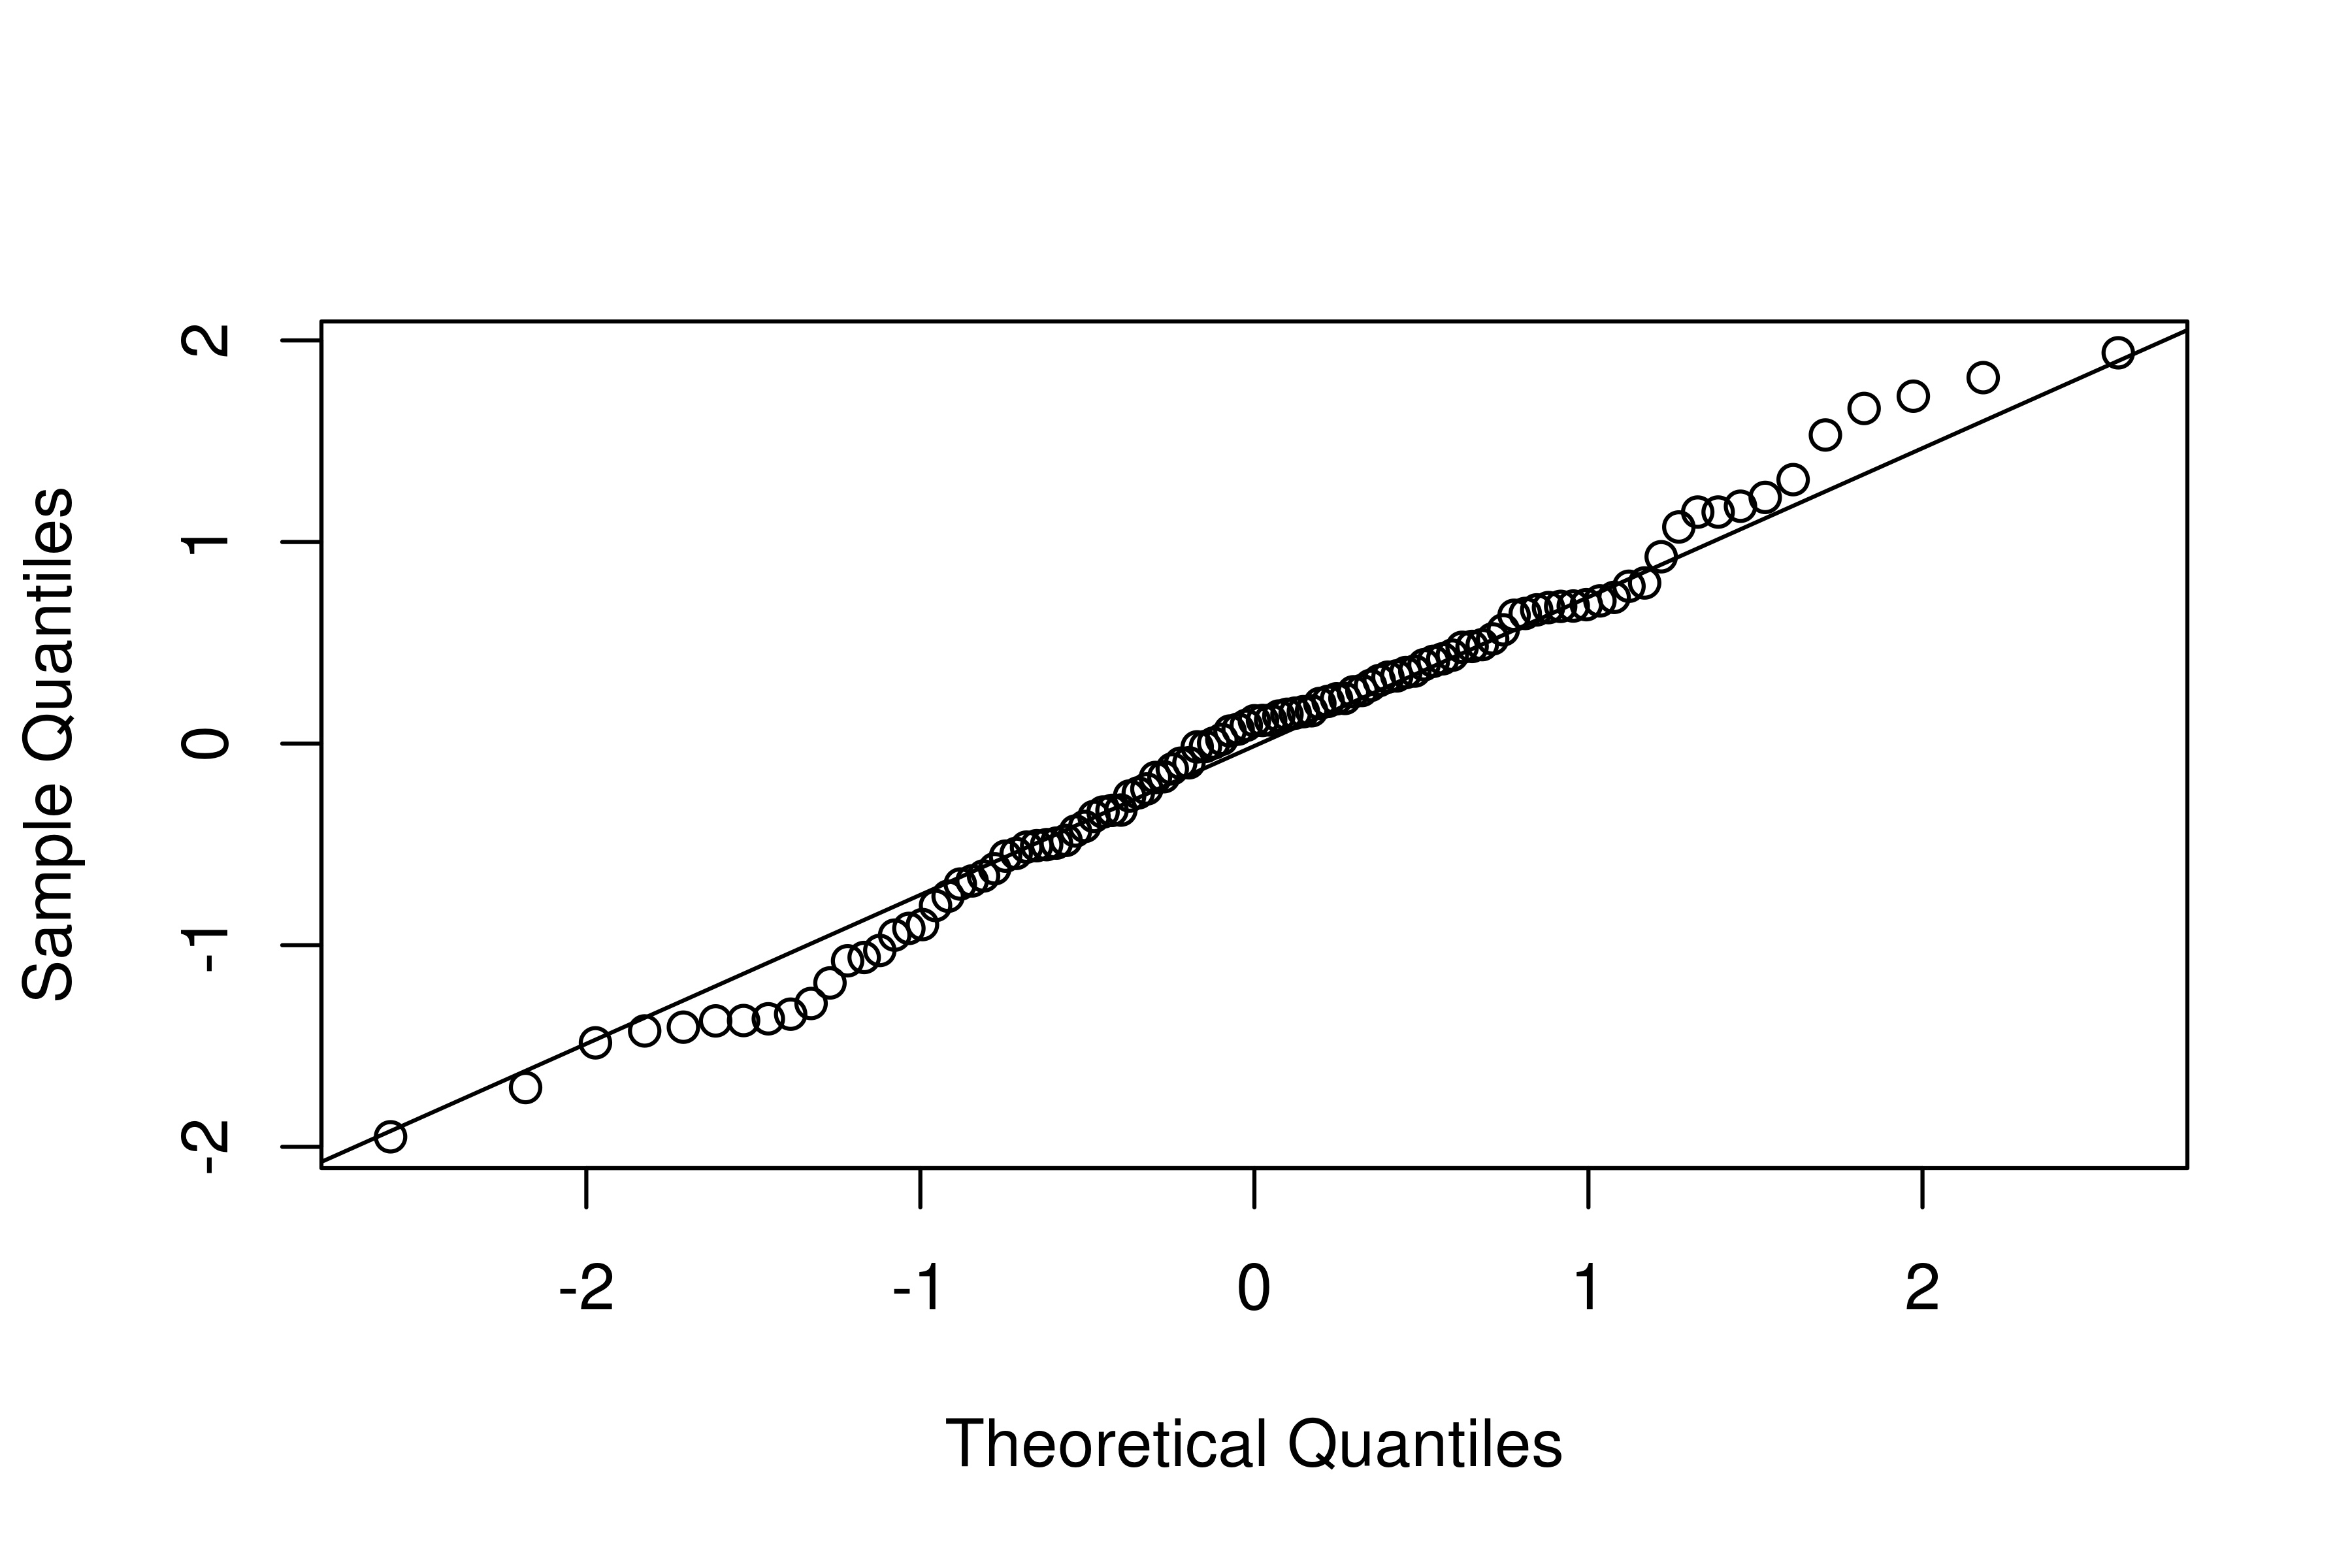
\includegraphics[width=.60\textwidth,height=.30\textheight]{qqplot.jpg}
%	\caption{Normal qqplot}
%\end{figure}
\subsubsection{Shapiro-Wilk Normality Test}
We also used Shapiro-Wilk Test to find whether the error is normaly distributed at a given significance.
\begin{itemize}
	\item $H_0$: The error is normally distributed.
	\item $H_A$: The error is not normally distributed.
\end{itemize}
Accoding to R, the p-value of S-W test statistics is 0.5181. It is large enough for us to accept the null hypothesis, which
means the error is normally distributed under any significance we usually use.
\subsubsection{Conclusion}
Our final model obeys the assumption $\varepsilon\sim \mathcal N(0,\sigma_{\varepsilon})$.  
\subsection{Constant Variance}
The assumption is that $\sigma_{\varepsilon}$ is constant in linear regression. There are two popular ways to verify this assumption, which are plotting $e_i v.s. \hat{y_i}$ and Fligner-Killeen  Test.
\subsubsection{$e_i$ v.s. $\hat{y_i}$ Plot}
Accoding to the figure in Figure3(b), there is similar pattern vertical spread across the plot, so we concluded that the variance is constant.
% \begin{figure}[H]
%	\centering
%	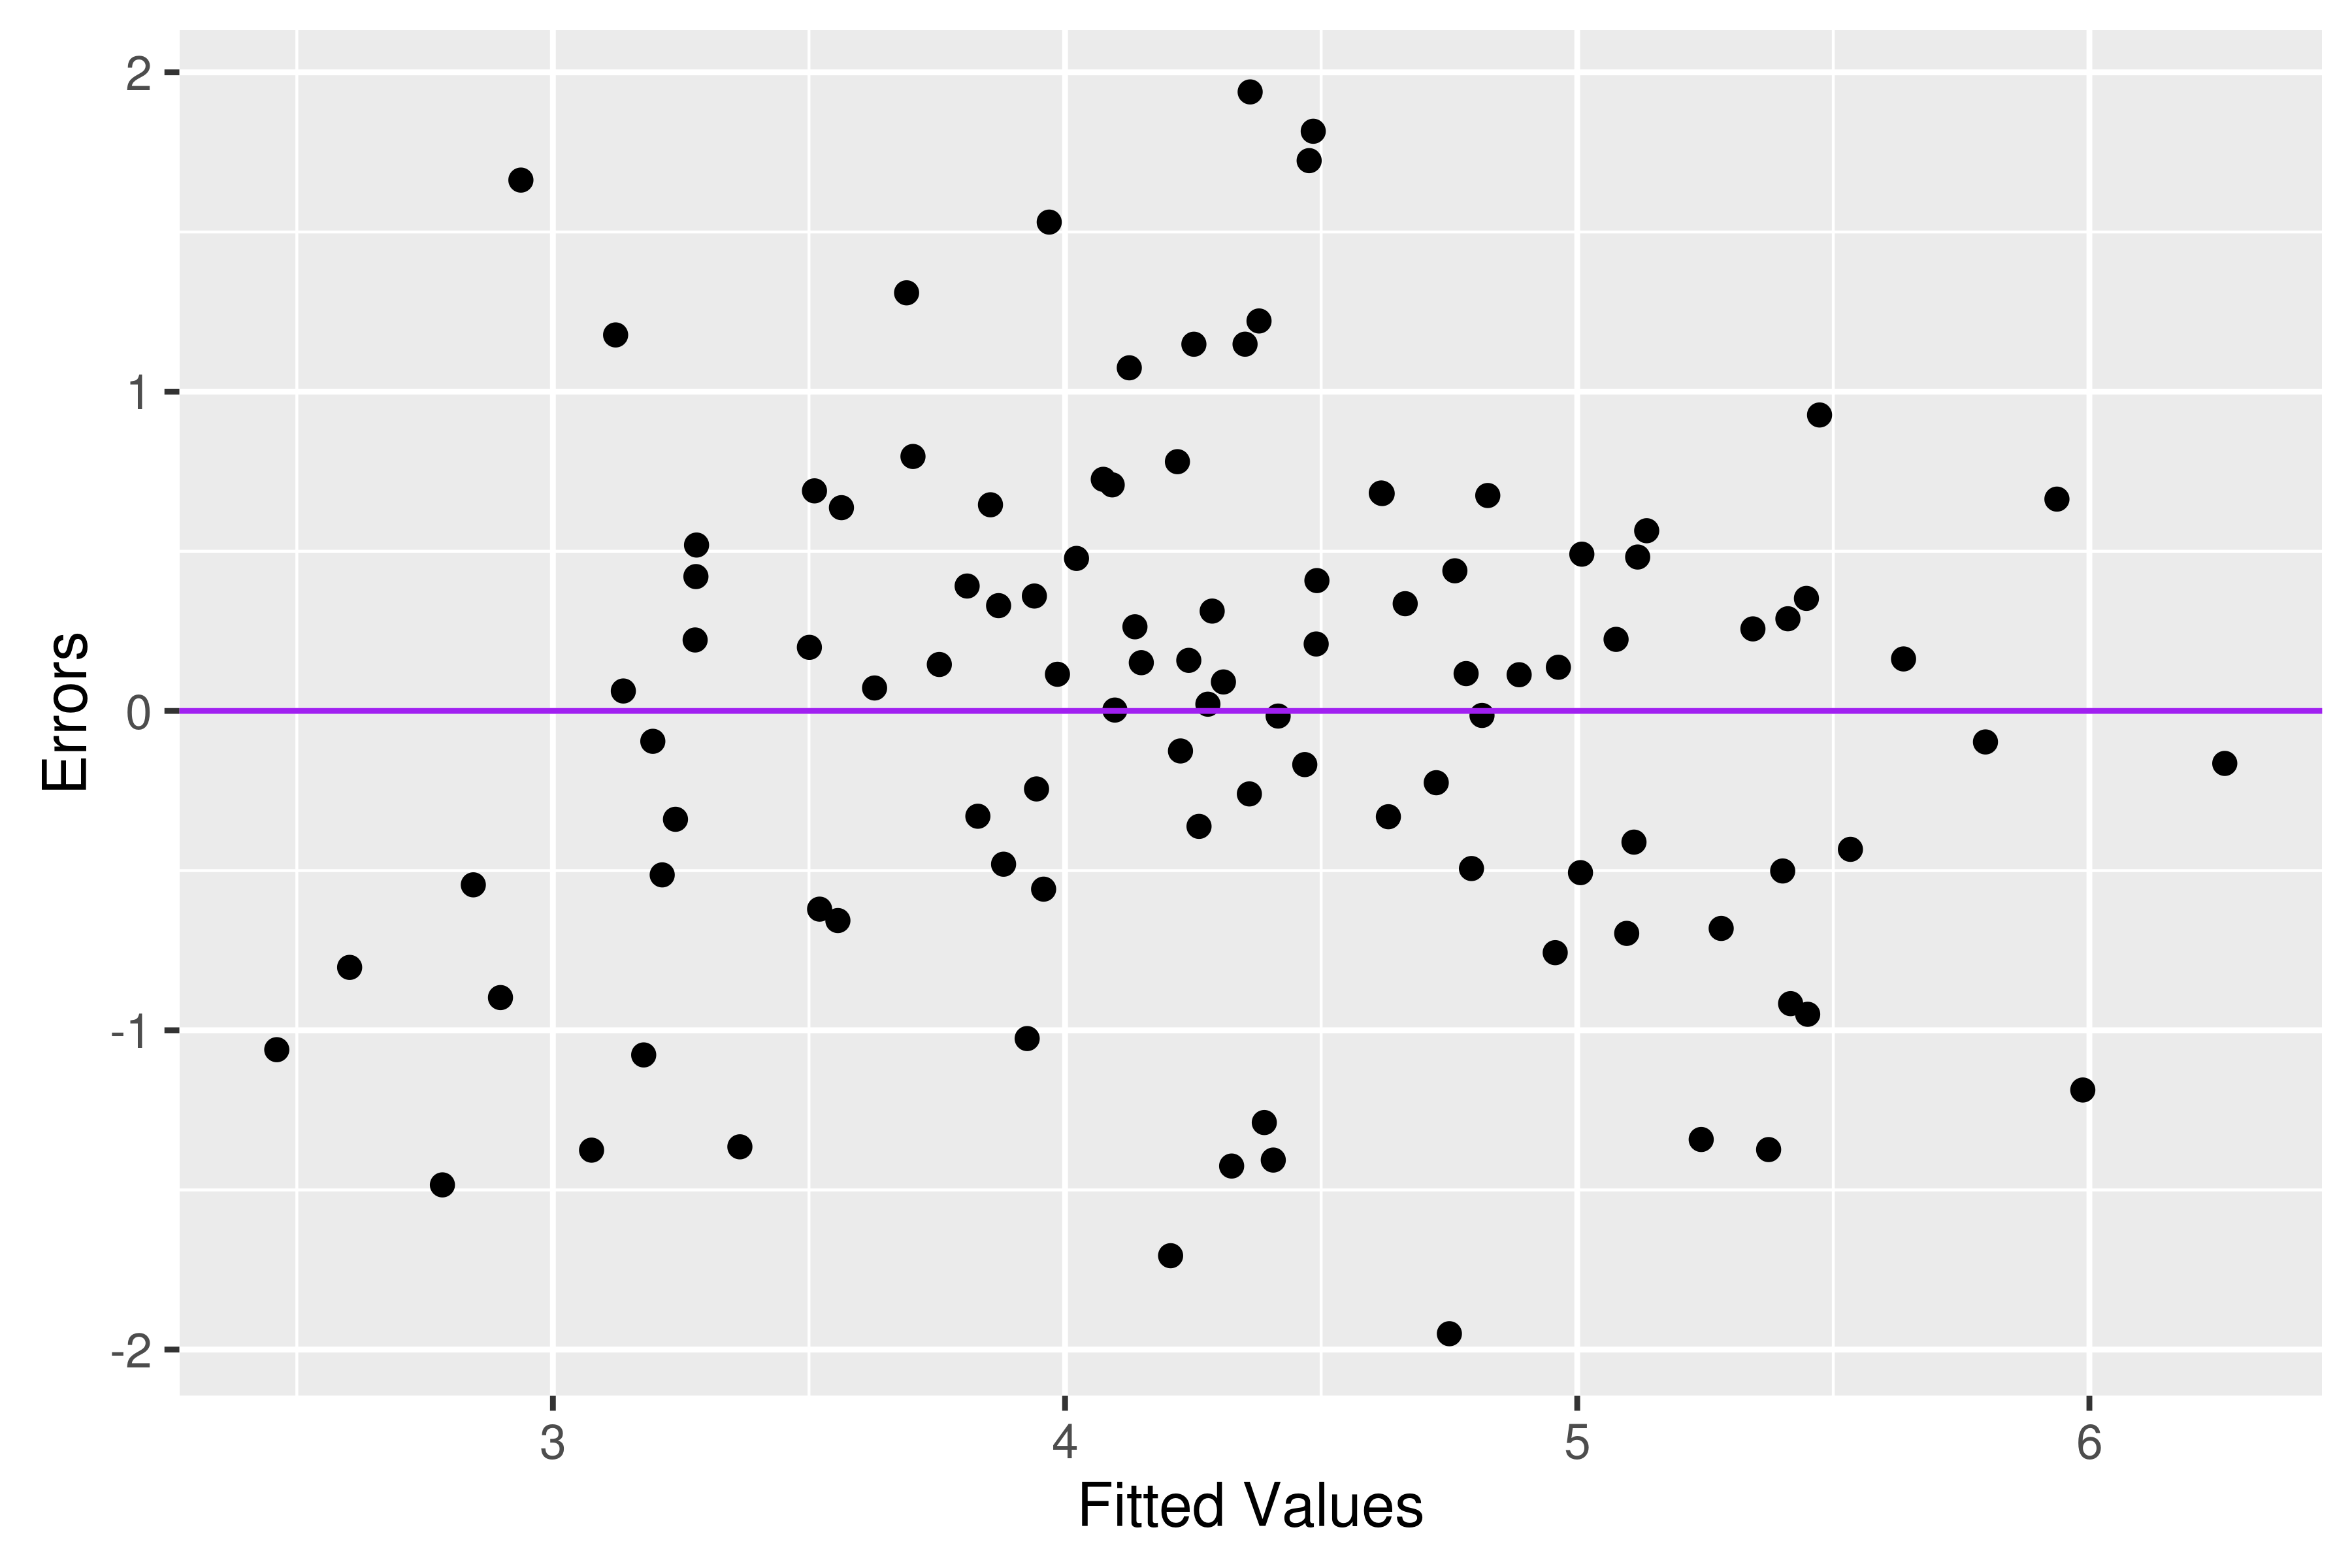
\includegraphics[width=.60\textwidth,height=.30\textheight]{scatter_plot_constant_variance.png} %1.png是图片文件的相对路径
%	\caption{$e_i$ v.s. $\hat{y_i}$} %caption是图片的标题
%	\label{img} %此处的label相当于一个图片的专属标志,目的是方便上下文的引用
%\end{figure}
\subsubsection{Fligner-Killeen  Test}
We used Fligner-Killeen Test to find whether the variance is constant.
\begin{itemize}
	\item $H_0$: $\sigma^2_{lower}=\sigma^2_{upper}$.
	\item $H_A$: $\sigma^2_{lower}\neq\sigma^2_{upper}$.
\end{itemize}
Accoding to R, the p-value of F-K test statistics is 0.2361. It is large enough for us to accept the null hypothesis, which
means the variance is constant under any significance we usually use.
\subsubsection{Conclusion}
Our final model obeys the assumption that the variance is constant.
\subsection{Remove  Outliers Again}
We used the method ``Cooks Distance" to find whether there are still some outliers in the dataset. As shown in the figure below, The ``Cooks Distance" is so small (less than the frequently used cutoff = 0.50) that there is no need to remove any points out of the current dataset.
 \begin{figure}[H]
	\centering
	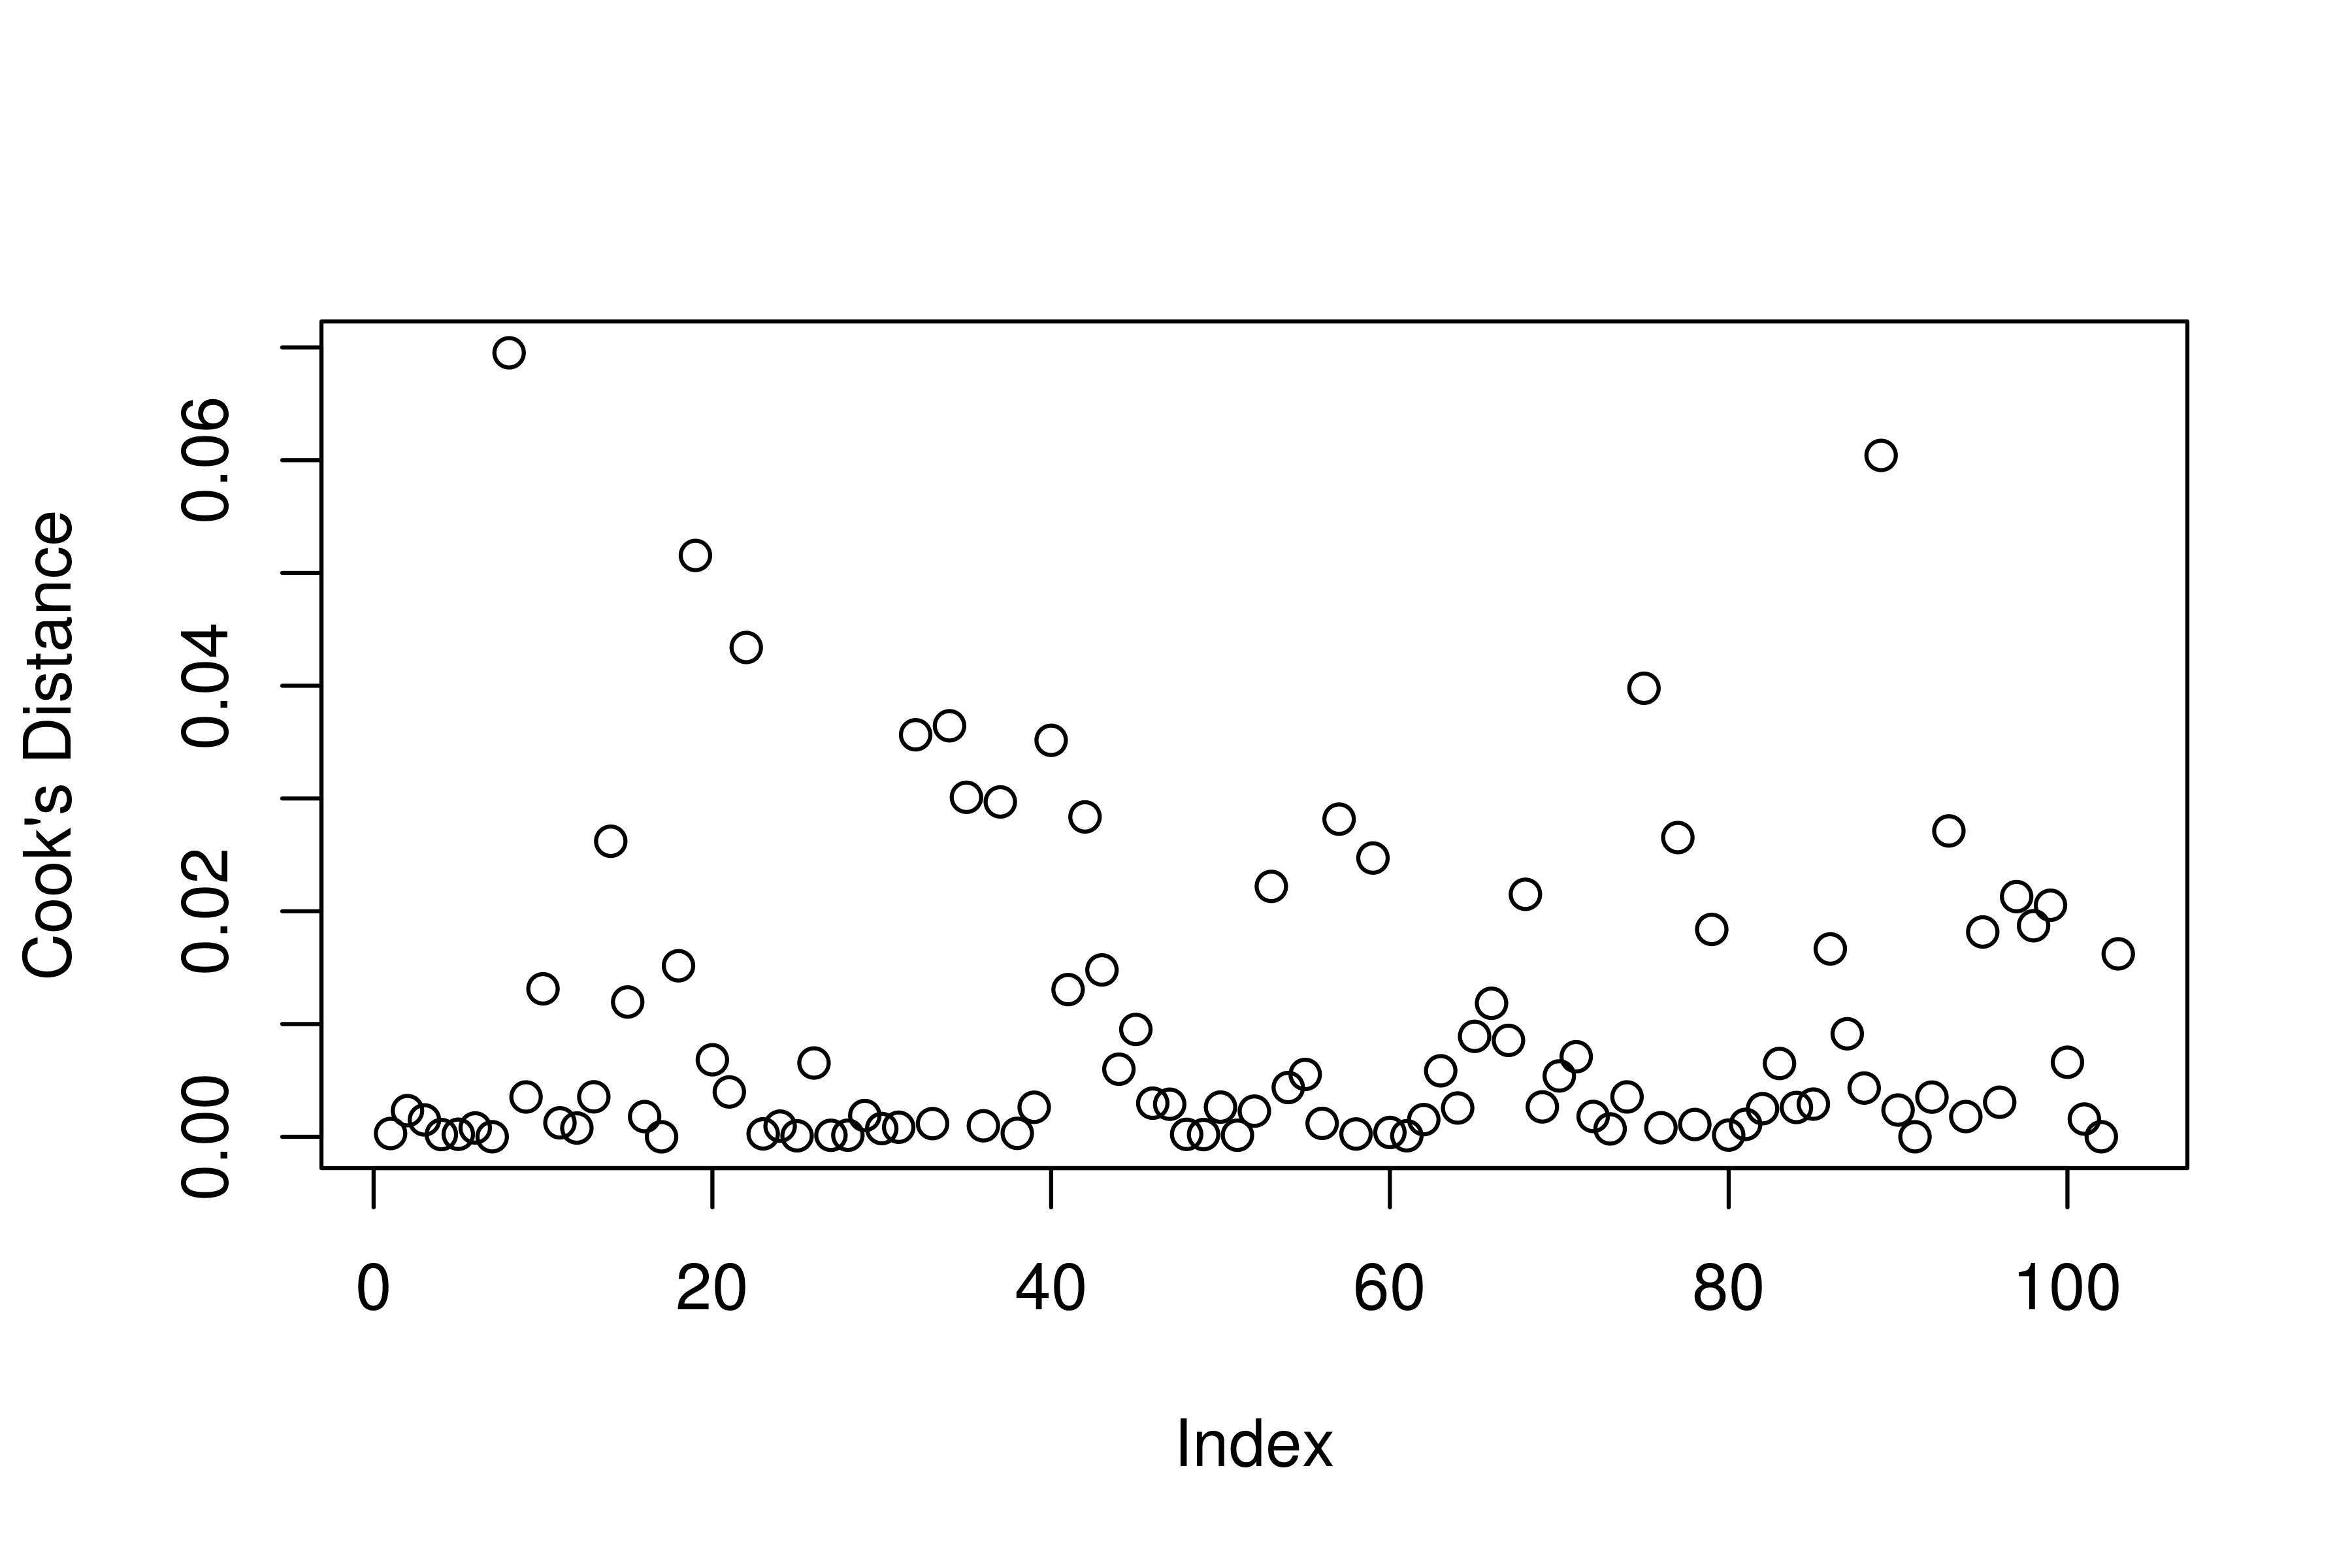
\includegraphics[width=.60\textwidth,height=.30\textheight]{cooks_distance.png} %1.png是图片文件的相对路径
	\caption{cook's distance} %caption是图片的标题
	\label{img} %此处的label相当于一个图片的专属标志,目的是方便上下文的引用
\end{figure}
\subsection{Final model}
Our final model is a ``correct"" model and it is appropriate, obeying linear regression assumptions, and there's no need to include interaction terms.
\begin{equation}
\begin{split}
Y= &-0.5573+0.4389X_1+0.0565X_2-0.5097X_{5NE}\\&-0.3471X_{5S}+0.9048X_{5W} +\varepsilon
\end{split}
\end{equation}
\par
This model can be written to four parallel lines due to the categorical variable $X_5$ and no interaction terms.
\begin{table}[H]
	\centering
	\begin{tabular}{cc}
		\midrule[1.5pt]	
		Category& Linear Regression function\\
		\hline    
		North Central&$\hat{y}=-0.5573+0.4389X_1+0.0565X_2$\\
		North East&$\hat{y}=-1.0670+0.4389X_1+0.0565X_2$\\
		South&$\hat{y}=-0.9044+0.4389X_1+0.0565X_2$\\
		West&$\hat{y}=0.3475+0.4389X_1+0.0565X_2$\\
		\midrule[1.5pt]
	\end{tabular}
	\caption{Linear regression function for different regions}
\end{table}

\section{Interpretation}
In this section, the meaning of every single $\beta$ is interpreted according to this problem.
\begin{itemize}
	\item $\beta_{0}$: Since the probability of acquring infection in hospital cannot be negative, it is inappropriate to predict the probability of acquiring infection at all $X$'s equal 0.
	\item $\beta_1$: When the length of stay of all patients in the hospital increases by 1 day, the probability of acquring infection in hospital tends to increase by 0.4389 percentage on average, holding all other variables constant.
	\item $\beta_2$: When the ratio of number of cultures performed to number of patients increases by 1, the probability of acquring infection in hospital tends to increase by 0.05648 percentage on average, holding all other variables constant.
	\item $\beta_{3}$: The probability of acquring infection in hospital tends to decrease by 0.5097 percentage on average when patients are in category of North East compared to patients in category of North Central, holding all other variables constant.
	\item $\beta_{4}$: The probability of acquiring infection in hospital tends to decrease by 0.3471 percentage on average when patients are in category of South compared to patients in category of North Central, holding all other variables constant.
	\item $\beta_{5}$: The probability of acquiring infection in hospital tends to increase by 0.9048 percentage on average when patients are in category of West compared to patients in category of North Central, holding all other variables constant.
	
\end{itemize}
\section{Prediction}
We used our final model to answer this question, 
``Predict the probability of infection in hospital with Stay=8, Culture=14, Region=`W'. "

\begin{table}[H]
	\centering
	\begin{tabular}{ccc}
		\midrule[1.5pt]	
		&point estimate &prediction intervals\\
		\hline
		$\bar{y}^{*}$&4.6493 	&[4.2042, 5.0945]\\
		$y^{*}$&4.6493			&[2.9272, 6.3715]\\
		\midrule[1.5pt]
	\end{tabular}
	\caption{Estimated value of Infect for $x^{*}$}
\end{table}
\section{Conclusion}
We have found that the average length of stay of all patients in the hospital($X_1$), the ratio of number of cultures performed to number of patients($X_2$) and geographical region($X_5$) have the most important effect on the prabability of acquiring infection in hospital.
\newpage
\section*{R Appendix}				
\begin{lstlisting}[language=R,caption={R script for Project 1}] 
##### set work directory and load dataset ##### 
setwd("/home/xmy/STA 101/Projects/P1")
HospFull<-read.csv("HospFull.csv", header = TRUE)
head(HospFull, n = 3)

##### load packages #####
library("ggplot2")
library("leaps")
library("MPV")

##### define functions #####
Partial.R2 = function(small.model,big.model){
SSE1 = sum(small.model$residuals^2)
SSE2 = sum(big.model$residuals^2)
PR2 = (SSE1 - SSE2)/SSE1
return(PR2)
}
All.Criteria = function(the.model){
p = length(the.model$coefficients)
n = length(the.model$residuals)
the.BIC = BIC(the.model)
the.LL = logLik(the.model)
the.AIC = AIC(the.model)
the.PRESS = PRESS(the.model)
the.R2adj = summary(the.model)$adj.r.squared
# the.CP = summary(the.model)$cp
the.results = c(the.LL,p,n,the.AIC,the.BIC,the.PRESS,the.R2adj)
names(the.results) = c("LL","p","n","AIC","BIC","PRESS","R2adj")
return(the.results)
}


##### correlation #####
cor(HospFull$Length, HospFull$Infect)
cor(HospFull$Culture, HospFull$Infect)
cor(HospFull$Bed, HospFull$Infect)


##### Infect summary #####
summary(HospFull$Infect)
# grouped by MedSchool
aggregate(Infect ~ MedSchool, data = HospFull, summary)
# grouped by Region
aggregate(Infect ~ Region, data = HospFull, summary)

# plot(HospFull)
##### boxplots of Infect #####
require(ggplot2)
# boxplot grouped by MedSchool
ppi = 600
# Calculate the height and width (in pixels) for a 4x3-inch image at 600 ppi
png("group_boxplot_medschool.png", width=6*ppi, height=4*ppi, res=ppi)
ggplot(HospFull, aes(y=Infect, x = MedSchool))+ theme_gray() + geom_boxplot() + ylab("Probability of acquiring infection in hospital") + 
xlab("category of MedSchool")+ coord_flip() 
#ggtitle("Boxplot of Infect grouped by Medchool") 
dev.off()

# boxplot grouped by Region
png("group_boxplot_region.png", width=6*ppi, height=4*ppi, res=ppi)
ggplot(HospFull, aes(y=Infect, x = Region))+ theme_gray() + geom_boxplot() + ylab("Probability of acquiring infection in hospital") + 
xlab("category of Geographical region")+ coord_flip() 
#ggtitle("Boxplot of Infect grouped by Region") 
dev.off()


##### scatter plots of Infect #####
# scatter plot of Infect vs. Length
png("scatter_plot_length.png", width=6*ppi, height=4*ppi, res = ppi)
qplot(HospFull$Length, HospFull$Infect, data = HospFull) +xlab("length of stay") + ylab("probability of acquiring infection")
dev.off()

# scatter plot of Infect vs. Culture
png("scatter_plot_culture.png",  width=6*ppi, height=4*ppi, res = ppi)
qplot(HospFull$Culture, HospFull$Infect, data = HospFull) +xlab("culture/patients * 100") + ylab("probability of acquiring infection")
dev.off()

# scatter plot of Infect vs. Bed
png("scatter_plot_bed.png", width=6*ppi, height=4*ppi, res = ppi)
qplot(HospFull$Bed, HospFull$Infect, data = HospFull) +xlab("number of beds") + ylab("probability of acquiring infection")
dev.off()



##### remove outliers according to plots #####
# cover HospFull
the.original = HospFull
HospFull=HospFull[-which(HospFull$Length>15),]
HospFull=HospFull[-which(HospFull$Culture>60),]
HospFull=HospFull[-which(HospFull$MedSchool=="Y" & HospFull$Infect > 7),]
HospFull=HospFull[-which(HospFull$MedSchool=="N" & HospFull$Infect > 7),]
HospFull=HospFull[-which(HospFull$Region=="W" & HospFull$Infect < 3),]
HospFull=HospFull[-which(HospFull$Region=="NC" & HospFull$Infect < 2),]
length(the.original$Infect)
length(HospFull$Infect)
the.ratio = (length(the.original$Infect)-length(HospFull$Infect))/length(the.original$Infect)
the.ratio

##### subset models of Infect~. #####
# rename dataset for convenience
names(HospFull) = c("X1","Y","X2","X3","X4","X5")
full.model = lm(Y~ X1 + X2 + X3 + X4 + X5,data = HospFull)
round(full.model$coefficients,4)
bic.model = lm(Y~X1+X2+X5, data = HospFull)
round(bic.model$coefficients, 4)
all.models = c("Y~1","Y~X1","Y~X2","Y~X3","Y~X4","Y~X5",
"Y~X1+X2","Y~X1+X3","Y~X1+X4","Y~X1+X5","Y~X2+X3","Y~X2+X4","Y~X2+X5","Y~X3+X4","Y~X3+X5","Y~X4+X5",
"Y~X1+X2+X3","Y~X1+X2+X4","Y~X1+X2+X5","Y~X1+X3+X4","Y~X1+X3+X5","Y~X1+X4+X5","Y~X2+X3+X4","Y~X2+X3+X5","Y~X2+X4+X5","Y~X3+X4+X5",
"Y~X1+X2+X3+X4","Y~X1+X2+X3+X5","Y~X1+X2+X4+X5","Y~X1+X3+X4+X5","Y~X2+X3+X4+X5",
"Y~X1+X2+X3+X4+X5")
Infect.all.model.crit = t(sapply(all.models,function(M){
current.model = lm(M,data = HospFull)
All.Criteria(current.model)
}))
Infect.all.model.crit
Infect.all.model.crit = data.frame(Infect.all.model.crit)
# find the model with lowest BIC
Infect.all.model.crit[which(Infect.all.model.crit$BIC == min(Infect.all.model.crit[,5])),]
# find the model with lowest AIC
Infect.all.model.crit[which(Infect.all.model.crit$AIC == min(Infect.all.model.crit[,4])),]


##### anova analysis of X4 #####
summary(full.model)
summary(bic.model)
alpha = 0.05
the.CIs = confint(full.model,level = 1-alpha)
round(the.CIs, 4)
# drop X4
smaller.model = lm(Y~X1+X2+X3+X5, data = HospFull)
anova.small = anova(smaller.model)
larger.model = lm(Y~X1+X2+X3+X4+X5, data = HospFull)
anova.large = anova(larger.model)
anova(smaller.model,larger.model)


##### anova analysis of X3 #####
smaller.model = lm(Y~X1+X2+X5, data = HospFull)
anova.small = anova(smaller.model)
larger.model = lm(Y~X1+X2+X3+X5, data = HospFull)
anova.large = anova(larger.model)
anova(smaller.model,larger.model)
##### partial r2 of X3 #####
partial.R2=Partial.R2(smaller.model, larger.model)
partial.R2


##### considering interaction terms #####
# interaction term between X1 and X5
final.model = lm(Y~X1+X2+X5, data = HospFull)
final.model
X1.interation.model = lm(Y~X1+X2+X5+X1*X5, data = HospFull)
summary(X1.interation.model)
confint(X1.interation.model,level = 1-alpha)
anova(final.model,X1.interation.model)
partial.R2=Partial.R2(final.model,X1.interation.model)
partial.R2
# interaction term between X2 and X5
X2.interation.model = lm(Y~X1+X2+X5+X2*X5, data = HospFull)
X2.interation.model
summary(X2.interation.model)
confint(X2.interation.model,level = 1-alpha)
anova(final.model,X2.interation.model)
partial.R2=Partial.R2(final.model,X2.interation.model)
partial.R2


##### diagnose of model #####
final.model = lm(Y~X1+X2+X5, data = HospFull)
final.model
HospFull$ei = final.model$residuals
HospFull$yhat = final.model$fitted.values
## nomality
# qqplot
png("qqplot.png", width=6*ppi, height=4*ppi, res = ppi)
qqnorm(final.model$residuals)
qqline(final.model$residuals)
dev.off()
# S-W test
the.SWtest = shapiro.test(final.model$residuals)
the.SWtest

## constant variance
# ei-yi plot
png("scatter_plot_constant_variance.png", width=6*ppi, height=4*ppi, res = ppi)
qplot(yhat, ei, data = HospFull) +
xlab("Fitted Values") + ylab("Errors") + geom_hline(yintercept = 0,col = "purple")
dev.off()
# F-K test
HospFull$ei = final.model$residuals
Group = rep("Lower",nrow(HospFull))
Group[HospFull$Y < median(HospFull$Y)] = "Upper"
Group = as.factor(Group)
HospFull$Group = Group
the.FKtest= fligner.test(HospFull$ei, HospFull$Group)
the.FKtest

## outliers
# cook's distance
cutoff = 0.10
CD = cooks.distance(final.model)
HospFull$CD = cooks.distance(final.model)
HospFull[which(HospFull$CD>cutoff),] 
# no outliers
png("cooks_distance.png", width=6*ppi, height=4*ppi, res = ppi)
plot(CD,ylab = "Cook's Distance")
abline(h = cutoff,color = "purple")
dev.off()

SR = stdres(final.model)
HospFull$SR = SR
cutoff= 3
png("standardized_error.png", width=6*ppi, height=4*ppi, res = ppi)
ggplot(HospFull,aes(x = SR))+geom_histogram(binwidth = 0.5,color = "black",fill = "white")+ xlab("standardized error")
dev.off()
SR[which(abs(SR) > cutoff)] 

##### final model #####
final.model
R2 = summary(final.model)$r.squared
R2

##### predict estimated values of Y #####
alpha = 0.05
x.star = data.frame(X1 = 8, X2 = 14, X5 = "W")
predict(final.model, x.star, interval = "confidence", level = 1-alpha)
predict(final.model, x.star, interval = "prediction", level = 1-alpha)
\end{lstlisting} 



\end{document}